\documentclass[a4paper, oneside, dvipsnames, table]{article}
\usepackage{../../Utilita/Stiletemplate}
\usepackage{hyperref}
\usepackage{fancyhdr}
\usepackage[italian]{babel}
\usepackage[raggedright]{titlesec}
\usepackage{blindtext}
\usepackage{amsmath}

\titleformat{\paragraph}[hang]{\normalfont\normalsize\bfseries}{\theparagraph}{1em}{}
\titlespacing*{\paragraph}{0pt}{3.25ex plus 1ex minus .2ex}{0.5em}

\setcounter{tocdepth}{5}
\setcounter{secnumdepth}{5}

\newcommand{\Titolo}{Piano di Qualifica}

\newcommand{\Redattori}{\AT{} \newline \MC{} \newline \BR{}}

\newcommand{\Verificatori}{\LD{} \newline \DF{}}

\newcommand{\Approvatore}{\SE{}}

\newcommand{\Distribuzione}{\Proponente{} \newline \VT{} \newline \CR{} \newline Gruppo \Gruppo{}}

\newcommand{\Uso}{Esterno}

\newcommand{\DescrizioneDoc}{Questo documento si occupa di descrivere il \PdQ{} realizzato dal Gruppo \Gruppo{} per il progetto \NomeProgetto{}.}

\newcommand{\pathimg}{../../Utilita/Immagini/qbteam.png}

\newcommand{\Versionedoc}{2.0.0}
% scritto da \DF{},\AT{}

% info generali 
\newcommand{\NomeProgetto}{\textit{Stalker}}

% fornitore
\newcommand{\Gruppo}{\textit{qbteam}}
\newcommand{\Mail}{qbteamswe@gmail.com}
% \newcommand{\pathimg}{Immagini/qbteam.png}

% committenti
\newcommand{\Committente}{\VT \newline \CR}
\newcommand{\VT}{Prof. Vardanega Tullio}
\newcommand{\CR}{Prof. Cardin Riccardo}

% proponenti
\newcommand{\Proponente}{\textit{Imola Informatica}}
\newcommand{\ZD}{Zanetti Davide}
\newcommand{\CT}{Cardona Tommaso}

% qbteam
\newcommand{\AT}{Azzalin Tommaso}
\newcommand{\DF}{Drago Francesco}
\newcommand{\BR}{Baratin Riccardo}
\newcommand{\MC}{Mattei Christian}
\newcommand{\PF}{Perin Federico}
\newcommand{\CE}{Cisotto Emanuele}
\newcommand{\SE}{Salmaso Enrico}
\newcommand{\LD}{Lazzaro Davide}

% ruoli
\newcommand{\Responsabile}{Responsabile di Progetto}
\newcommand{\Amministratore}{Amministratore di Progetto}

% documenti

\newcommand{\SdF}{Studio di Fattibilità}
\newcommand{\SdFv}[1]{\textit{Studio di Fattibilità {#1}}}
\newcommand{\PdQ}{Piano di Qualifica}
\newcommand{\PdQv}[1]{\textit{Piano di Qualifica {#1}}}
\newcommand{\PdP}{Piano di Progetto}
\newcommand{\PdPv}[1]{\textit{Piano di Progetto {#1}}}
\newcommand{\NdP}{Norme di Progetto}
\newcommand{\NdPv}[1]{\textit{Norme di Progetto {#1}}}
\newcommand{\AdR}{Analisi dei Requisiti}
\newcommand{\AdRv}[1]{\textit{Analisi dei Requisiti {#1}}}
\newcommand{\Glossario}{Glossario}
\newcommand{\Glossariov}[1]{\textit{Glossario {#1}}}
\newcommand{\MM}{Manuale Manutentore}
\newcommand{\MU}{Manuale Utente}

% comandi generali
\newcommand{\glo}[1]{#1\ap{G}}

\setlength{\parindent}{-0.1em}

\begin{document}

\copertina{}
\fancydoc{}
\newpage
\section*{Registro delle modifiche}
{
\rowcolors{2}{grigetto}{white}
\renewcommand{\arraystretch}{1.5}
\centering
\begin{longtable}{ c c  C{2.3cm} c C{3cm} C{3.2cm}}
\rowcolor{rossoep}
\textcolor{white}{\textbf{Versione}} & \textcolor{white}{\textbf{Data}} & \textcolor{white}{\textbf{Nominativo}} & \textcolor{white}{\textbf{Ruolo}} & 
\textcolor{white}{\textbf{Verificatore}}& \textcolor{white}{\textbf{Descrizione}}\\	


1.0.0 & \Data & \CE{} & Responsabili & \CE{} & Approvazione per il rilascio.  \\
		
0.0.1 & \Data & \DF{} & Analista & \AT{} & Stesura e verifica del documento.  \\
		
		
\end{longtable}
}

\clearpage
\tableofcontents
\clearpage

\setcounter{table}{0}

\renewcommand{\listtablename}{Elenco tabelle}

\listoffigures
\clearpage
\listoftables
\clearpage

% scritto da\AT{}
\section{Introduzione}
\subsection{Scopo del documento}
Il presente documento ha lo scopo di descrivere le strategie che il gruppo \Gruppo{} intende applicare per garantire la qualità di processo e di prodotto per l’intera durata del progetto.
Al fine di rispettare questi obiettivi vengono descritte le modalità in cui vengono effettuate la verifica e la validazione del prodotto.
In questo modo è consentita la rilevazione e correzione di problemi o incongruenze in breve tempo, senza correre il rischio di sprechi di risorse.

\subsection{Scopo generale del prodotto}
L'obiettivo del prodotto \NomeProgetto{} di \Proponente{} è la creazione di un sistema software composto di un applicativo per cellulare e di un server, con cui interagire tramite un'interfaccia utente. La necessità nasce dal bisogno di adempiere alle normative vigenti in tema di sicurezza.
Le due componenti del sistema software, applicativo e server, devono soddisfare i seguenti obiettivi rispettivamente di:
\begin{itemize}
\item Tracciare e registrare i \glo{movimenti} di un utente in un \glo{luogo di tracciamento} di un'\glo{organizzazione}, siano essi autenticati da credenziali di un'\glo{organizzazione} oppure visitatori anonimi, il tutto nel rispetto della normativa sulla privacy;
\item Poter visionare gli accessi degli utenti autenticati e visionare il numero di visitatori anonimi all'interno di un luogo.
\end{itemize}

\subsection{Glossario}
Al fine di evitare ambiguità fra i termini, e per avere chiare fra tutti gli stakeholder le terminologie utilizzate per la realizzazione del presente documento, il gruppo \Gruppo{} ha redatto un documento denominato \Glossariov{1.0.0}.
In tale documento, sono presenti tutti i termini tecnici, ambigui, specifici del progetto e scelti dai membri del gruppo con le loro relative definizioni.
Un termine presente nel \Glossariov{1.0.0} e utilizzato in questo documento viene indicato con un apice \ap{G} alla fine della parola.

\subsection{Standard di progetto}
Il gruppo \Gruppo{} ha deciso di gestire i propri processi del ciclo di vita del software adottando alcune parti dello standard \textbf{ISO/IEC 12207} come definito nelle \textit{NormeDiProgetto}; 
come modello di qualità del prodotto software si è utilizzato parte dello standard \textbf{ISO/IEC 9126} anch'esso definito nelle \textit{NormeDiProgetto}.

\subsection{Riferimenti}

\subsubsection{Normativi}
\begin{itemize}
    \item \textbf{Capitolato d'appalto C5 - Stalker}\\     
    \url{https://www.math.unipd.it/~tullio/IS-1/2019/Progetto/C5.pdf};
    \item \NdPv{1.0.0}.
    \item \textbf{ISO/IEC 12207-1995:}\\     
    \url{https://www.math.unipd.it/~tullio/IS-1/2009/Approfondimenti/ISO_12207-1995.pdf};\\
    \url{http://www.colonese.it/SviluppoSw_Standard_ISO12207.html};
    \item \textbf{ISO/IEC 9126:}\\
    \url{http://www.colonese.it/00-Manuali_Pubblicatii/07-ISO-IEC9126_v2.pdf};\\
    \url{https://en.wikipedia.org/wiki/ISO/IEC_9126};
\end{itemize}

\subsubsection{Informativi}
\begin{itemize}
    \item \textbf{Indice di Gulpease}\\
    \url{https://it.wikipedia.org/wiki/Indice_Gulpease};
    \item \textbf{Metriche di progetto}\\
    \url{https://it.wikipedia.org/wiki/Metriche_di_progetto};
    \item \textbf{Varie metriche}\\
    \url{http://torlone.dia.uniroma3.it/sistelab/annipassati/sbavaglia.pdf};
    \item \textbf{Ciclo di Deming - Plan Do Check Act}\\
    \url{https://it.wikipedia.org/wiki/Ciclo_di_Deming};
    
\end{itemize}
\newpage
\section{Qualità di processo}
Per garantire la qualità dei processi\ap{G} si utilizza come riferimento lo standard ISO/IEC 12207:1995. Dopo uno studio dettagliato di tale documento sono stati scelti i processi\ap{G}
e le attività da utilizzare. Il tutto è stato semplificato ed adattato in base alle esigenze del progetto. Come è previsto nello standard, tutti i processi\ap{G} e le attività sono raccolti 
nei processi\ap{G}: primari, di supporto ed organizzativi. Le attività fanno parte a dei sotto processi\ap{G} rispetto a quelli appena elencati e per questo motivo la loro 
appartenenza è resa chiara nella sezione: Processo\ap{G} di riferimento.\\ \\
\textbf{Metriche di processo:}\\
Vengono utilizzate delle metriche che servono per monitorare lo stato dei processi scelti nello standard. Il Responsabile, grazie ai valori ricavati dalle metriche, è facilitato nel
valutare il processo e di eseguire modifiche alla pianificazione se necessario.\\ \\
Ogni metrica ha un codice univoco ed è strutturato in questo formato \textbf{MPC-00}:
\begin{itemize}
    \item \textbf{M}: metrica
    \item \textbf{PC}: processo
    \item \textbf{-} : trattino separatore
    \item \textbf{00}: numero incrementale
\end{itemize}

\subsection{Processi primari}
Sono i processi\ap{G} e le attività che fanno parte dello sviluppo del software e hanno lo scopo di soddisfare tutti i requisiti concordati con il cliente.

\subsubsection{Analisi dei requisiti}
    \paragraph{Metrica - Percentuale requisiti soddisfatti}
    \begin{itemize}
        \item \textbf{Codice:} MPC-01
        \item \textbf{Descrizione:} È la percentuale dei requisiti che devono essere soddisfatti.
        \item \textbf{Processo di riferimento:} Sviluppo
        \item \textbf{Sigla:} $PRS$
        \item \textbf{Formula:} $$PRS = {requisiti \; soddisfatti \over requisiti \; totali}\; \cdot \; 100$$
        \item \textbf{Range di valori che può assumere:}
        \begin{itemize}
            \item \textbf{Accettabile:} $PRS = 100\%$
            \item \textbf{Ottimale:} $PRS = 100\%$
        \end{itemize}
    \end{itemize}

\subsubsection{Progettazione di dettaglio}
\newpage %adattamento pdf
    \paragraph{Metrica - Incapsulamento CBO}
    \begin{itemize}
        \item \textbf{Codice:} MPC-02
        \item \textbf{Descrizione:} Il "Coupling Between Objects" misura il numero delle classi correlate ad una classe al di fuori dalla gerarchia di ereditarietà. Più è alto il grado di coupling e più il sistema è difficile da mantenere.
        \item \textbf{Processo di riferimento:} Sviluppo
        \item \textbf{Sigla:} $CBO$
        \item \textbf{Formula:} $$CBO = {\sum_{i=1}^{N} C_i}$$
        con:
        \begin{itemize}
            \item $N$ = numero classi non appartenenti alla gerarchia di ereditarietà
            \item $C_i$ = classe correlata
        \end{itemize}
        \item \textbf{Range di valori che può assumere:}
        \begin{itemize}
            \item \textbf{Accettabile:} $0 \leq{} CBO \leq 4$
            \item \textbf{Ottimale:} $0 \leq{} CBO \leq 2$
        \end{itemize}
    \end{itemize}

    \paragraph{Metrica - Livello profondità gerarchia}
    \begin{itemize}
        \item \textbf{Codice:} MPC-03
        \item \textbf{Descrizione:} È il valore intero che indica la profondità della gerarchia formata tra classi. Se una gerarchia è formata da una classe allora il valore è uguale a 1.
        \item \textbf{Processo di riferimento:} Sviluppo
        \item \textbf{Sigla:} $LPG$
        \item \textbf{Range di valori che può assumere:}
        \begin{itemize}
            \item \textbf{Accettabile:} $1 \leq{} LPG \leq 3$
            \item \textbf{Ottimale:} $1 \leq{} LPG \leq 2$
        \end{itemize}
    \end{itemize}

\subsubsection{Codifica}  
    \paragraph{Metrica - Numero di parametri per metodo} 
    \begin{itemize}
        \item \textbf{Codice:} MPC-04
        \item \textbf{Descrizione:} Un numero elevato di parametri per metodo può indicare il bisogno di ridurre funzionalità associate a tale metodo. Più è grande questo valore e più la possibilità aumenta nel commettere errori progettuali.
        \item \textbf{Processo di riferimento:} Sviluppo
        \item \textbf{Sigla:} $NPM$
        \item \textbf{Range di valori che può assumere:}
        \begin{itemize}
            \item \textbf{Accettabile:} $0 \leq{} NPM \leq 8$
            \item \textbf{Ottimale:} $0 \leq{} NPM \leq 4$
        \end{itemize}
    \end{itemize}

    \paragraph{Metrica - Linee di commento per linee di codice}
    \begin{itemize}
        \item \textbf{Codice:} MPC-05
        \item \textbf{Descrizione:} È il rapporto tra linee di commento e linee di codice. Per le linee di codice si intende Logical SLOC il numero di linee di codice effettive che corrispondono al numero di statement.
        \item \textbf{Processo di riferimento:} Sviluppo
        \item \textbf{Sigla:} $LCLC$
        \item \textbf{Formula:}$$LCLC = {linee \; di \; commento\over linee \; di \; codice}$$
        \item \textbf{Range di valori che può assumere:}
        \begin{itemize}
            \item \textbf{Accettabile:} $LCLC \geq 0.25$
            \item \textbf{Ottimale:} $LCLC \geq 0.30$
        \end{itemize}
    \end{itemize}

\subsection{Processi supporto}
Sono i processi\ap{G} e le attività che aiutano gli altri processi\ap{G} nel raggiungimento del successo e nella qualità del progetto.
  
\subsubsection{Implementazione}
    \paragraph{Metrica - Indice di Gulpease}
    \begin{itemize}
        \item \textbf{Codice:} MPC-06
        \item \textbf{Descrizione:} È l'indice di leggibilità di un determinato testo. Calcola la lunghezza delle parole e delle frasi rispetto al numero totale delle lettere. Il valore è un intero da 0 a 100; se esso è inferiore a 80 sarà difficile da leggere per chi ha la licenza elementare, mentre se è inferiore a 40 sarà difficili da leggere per chi ha un diploma superiore.
        \item \textbf{Processo di riferimento:} Documentazione
        \item \textbf{Sigla:} $IG$
        \item \textbf{Formula:} $$IG = 89 + {{300 \; \cdot \; (numero\; delle \; frasi) \; - \; 10 \; \cdot \; (numero \; delle \; lettere)}\over numero \; delle \; parole}$$
        \item \textbf{Range di valori che può assumere:}
        \begin{itemize}
            \item \textbf{Accettabile:} $40 < IG < 100$
            \item \textbf{Ottimale:} $80 < IG < 100$
        \end{itemize}
    \end{itemize}

\subsubsection{Garanzia}
    \paragraph{Metrica - Efficacia del processo}
    \begin{itemize}
        \item \textbf{Codice:} MPC-07
        \item \textbf{Descrizione:} Viene indicato se il processo\ap{G} rispetta gli effetti e i risultati voluti. Un processo\ap{G} deve essere efficace\ap{G} al 100\% per garantire la sua qualità.
        \item \textbf{Processo di riferimento:} Garanzia di qualità
        \item \textbf{Sigla:} $EP$
        \item \textbf{Range di valori che può assumere:}
        \begin{itemize}
            \item \textbf{Accettabile:} $EP = 100\%$
            \item \textbf{Ottimale:} $EP = 100\%$
        \end{itemize}
    \end{itemize}

\subsubsection{Verifica}
    \paragraph{Metrica - Code coverage}
    \begin{itemize}
        \item \textbf{Codice:} MPC-08
        \item \textbf{Descrizione:} È la percentuale di copertura del codice attraversato dai test rispetto al totale del codice di base. Per dare una misurazione in termini di grandezza si adoperano le linee di codice come riferimento.
        \item \textbf{Processo di riferimento:} Processi\ap{G} di verifica
        \item \textbf{Sigla:} $CC$
        \item \textbf{Formula:} $$CC = {linee \; di \; codice \; percorse \; dai  \; test \over linee \; di \; codice \; totali} \; \cdot \; 100$$
        \item \textbf{Range di valori che può assumere:}
        \begin{itemize}
            \item \textbf{Accettabile:} $CC = 80\%$
            \item \textbf{Ottimale:} $CC = 100\%$
        \end{itemize}
    \end{itemize}

\subsection{Processi organizzativi}
Sono i processi\ap{G} e le attività che coprono gli aspetti organizzativi e di gestione delle risorse.

\subsubsection{Pianificazione}
    \paragraph{Metrica - Schedule variance}
    \begin{itemize}
        \item \textbf{Codice:} MPC-09
        \item \textbf{Descrizione:} È il valore che indica se si è in linea ($=0$), in anticipo ($>0$) oppure in ritardo ($<0$) rispetto alla schedulazione delle attività di progetto pianificate nella baseline\ap{G}.
        \item \textbf{Processo di riferimento:} Gestione
        \item \textbf{Sigla:} $SV$
        \item \textbf{Formula:} $$SV = {BCWP \; - \; BCWS}$$
        con:
        \begin{itemize}
            \item $BCWP$ = Budgeted Cost of Work Performed (valore delle attività eseguite nella data corrente)
            \item $BCWS$ = Budgeted Cost of Work Scheduled (costo pianificato per la realizzazione delle attività di progetto alla data corrente)
        \end{itemize}
        \item \textbf{Range di valori che può assumere:}
        \begin{itemize}
            \item \textbf{Accettabile:} $SV = 0$
            \item \textbf{Ottimale:} $SV > 0$
        \end{itemize}
    \end{itemize}

    \paragraph{Metrica - Budget variance}
        \begin{itemize}
            \item \textbf{Codice:} MPC-10 
            \item \textbf{Descrizione:} È il valore che indica se la data corrente si è speso di più ($>0$) o di meno ($<0$) rispetto a quanto pianificato dal budget totale $B_{tot}$.
            \item \textbf{Processo di riferimento:} Gestione
            \item \textbf{Sigla:} $BV$
            \item \textbf{Formula:} $$BV = {BCWS \; - \; ACWP}$$
            con:
            \begin{itemize}
                \item $BCWS$ = Budgeted Cost of Work Scheduled (costo pianificato per la realizzazione delle attività di progetto alla data corrente)
                \item $ACWP$ = Actual Cost of Work Performed (costo effettivamente sostenuto alla data corrente)
                \item $B_{tot}$ = Budget totale
            \end{itemize}
            \item \textbf{Range di valori che può assumere:}
            \begin{itemize}
                \item \textbf{Accettabile:} $0 \leq BV < ACWP$
                \item \textbf{Ottimale:} $0 \leq BV \leq B_{tot}$
            \end{itemize}
        \end{itemize}

\subsection{Tabella metriche dei processi}
    \rowcolors{2}{grigetto}{white}
    \renewcommand{\arraystretch}{1.5}
    \begin{longtable}{ c C{4cm} c c c}
    \rowcolor{darkblue}
    \textcolor{white}{\textbf{Metrica}} & \textcolor{white}{\textbf{Nome}} & \textcolor{white}{\textbf{Sigla}} & \textcolor{white}{\textbf{Valore Accettabile}} & \textcolor{white}{\textbf{Valore Ottimale}}\\
    MPC-01 & Percentuale Requisiti Soddisfatti & $PRS$ & $PRS=100\%$ & $PRS=100\%$ \\
    MPC-02 & Coupling Between Objects & $CBO$ & $0 \leq CBO \leq 4$ & $0 \leq CBO \leq 2$ \\
    MPC-03 & Livello Profondità Gerarchia & $LPG$ &  $1 \leq LPG \leq 3$ &  $1 \leq LPG \leq 2$ \\
    MPC-04 & Numero di Parametri per Metodo & $NPM$ & $0 < NPM < 8$ & $ 0 < NPM < 4$ \\
    MPC-05 & Linee di Codice per Linee di Commento & $LCLC$ & $LCLC \geq 0.25$ & $LCLC \geq 0.30$ \\
    MPC-06 & Indice di Gulpease & $IG$ & $40 < IG < 100$ & $80 < IG < 100$ \\
    MPC-07 & Efficacia del Processo\ap{G} & $EP$ & $EP = 100\%$ & $EP = 100\%$ \\
    MPC-08 & Code Coverage & $CC$ & $CC = 80\%$ & $CC = 100\%$  \\
    MPC-09 & Schedule Variance & $SV$ & $SV = 0$ & $SV > 0$  \\	
    MPC-10 & Budget Variance & $BV$ & $0 \leq BV < ACWP$ & $0 \leq BV \leq B_{tot}$  \\
    \end{longtable}

\newpage %adattamento pdf

\subsection{Ciclo di Deming}
    Il ciclo di Deming è un metodo di gestione iterativo per il controllo e il miglioramento continuo dei processi (e anche dei prodotti) suddiviso in 4 fasi: Plan, Do, Check e Act. 
    Anche la norma ISO/IEC 12207 utilizza questo ciclo per scopi di miglioria dei processi\ap{G}. Per garantire la qualità dei processi\ap{G} e la coerenza allo standard, il gruppo qbteam 
    ha scelto di adottare il ciclo PDCA.

    \begin{figure}[h]
        \centering
        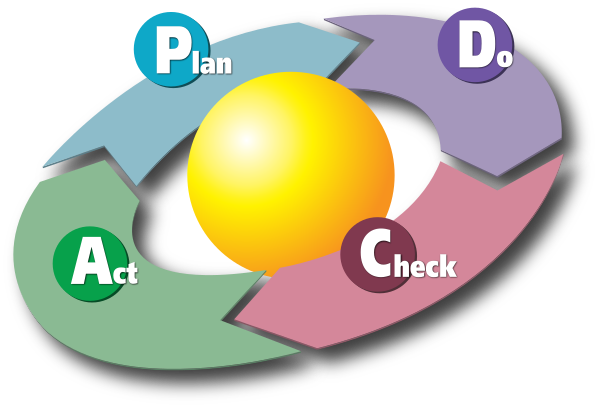
\includegraphics[scale=0.2]{sezioni/Immagini/PDCA.png}
        \caption{Ciclo PDCA - Plan Do Check Act}
    \end{figure}

    \textbf{Fasi del ciclo PDCA:}:
    \begin{itemize}
        \item \textbf{Plan}: definisce attività e scadenze necessarie al raggiungimento dei specifici obiettivi di miglioramento;
        \item \textbf{Do}: esegue le attività di "Plan";
        \item \textbf{Check}: verifica l'esito delle azioni di miglioramento rispetto alle attese. Si analizzano i risultati del "Do" e li si confrontano con gli obiettivi individuati nel "Plan";
        \item \textbf{Act}: consolida il tutto e cerca dei metodi per il prossimo miglioramento. Se il "Check" ha dimostrato che il "Plan" implementato dal "Do" è migliore rispetto ai precedenti processi\ap{G} standard, allora questo piano diventa il nuovo processo\ap{G} standard. Altrimenti il vecchio standard in uso rimarrà la baseline\ap{G}.
    \end{itemize}
\newpage

\section{Qualità di prodotto}
La qualità di un prodotto software è valutata secondo criteri semplici e comprensibili per tutti, utenti e sviluppatori, operatori e addetti alla manutenzione.
Per valutare tale qualità il gruppo "Qbteam" ha deciso di far riferimento allo standard ISO/IEC 9126, le quali norme descrivono:

\begin{itemize}
\item Un modello di qualità del software;
\item Le caratteristiche che determinano la qualità del software;
\item Le metriche per la misurazione della qualità del software;
\end{itemize}

In questa sezione di documento verranno riportate solo alcune delle caratteristiche definite dallo standard, ovvero quelle ritenute più inerenti ai fini del progetto.

\subsection{Metriche interne}
 Le metriche della qualità "interne" del software sono utilizzate durante la fase di sviluppo e permettono di valutare il comportamento del software dal punto di vista degli sviluppatori e di predire quello che sarà il punto di vista esterno degli utenti.
  \subsubsection{Funzionalità}
      Capacità del prodotto software di soddisfare i requisiti funzionali e le necessità degli utenti.\\

              \paragraph{Metrica - Aderenza delle funzioni e/o delle interfacce} 
              \begin{itemize}
          \item  \textbf{Codice:} MPD-01
        \item    \textbf{Descrizione:} Misurare il livello di aderenza delle funzioni e delle interfacce sviluppate rispetto agli standard, alle normative e alla regolamentazioni
          \item  \textbf{Attributo di riferimento:} Aderenza alle funzionalità 
        \item    \textbf{Sigla:} AFI
         \item   \textbf{Formula:} \begin{math}AFI = \frac{A}{B}\end{math}\\ \\
              A = numero di funzioni(e/o interfacce) sviluppate che risultano aderenti a standard, regole e normative emesse al riguardo; \\
              B = numero totale di funzioni(e/o interfacce) che devono essere aderenti a tali regole come descritto nelle specifiche;
                   \item \textbf{Range di valori che può assumere:}
        \begin{itemize}
            \item \textbf{Accettabile:} 
            \item \textbf{Ottimale:} 
        \end{itemize}
       \end{itemize}
              
  \subsubsection{Affidabilità} 
  Capacità di predire se il prodotto software in questione potrà soddisfare i requisiti prescritti per l'affidabilità dal punto di vista degli sviluppatori.\
                \paragraph{Metrica - Rilevamento dei difetti} 
                  \begin{itemize}
         \item   \textbf{Codice:} MPD-02
         \item   \textbf{Descrizione:} Misurare l'efficacia nel rilevare i difetti presenti nel software durante le diverse fasi di sviluppo del prodotto
        \item    \textbf{Attributo di riferimento:} Maturità
        \item    \textbf{Sigla:} RDF
        \item    \textbf{Formula:} \begin{math} RDF = \frac{A}{B}\end{math}\\ \\
             A = numero di difetti rilevati nelle revisioni tecniche, ispezioni e test del prodotto in ciascuna fase di sviluppo;\\
              B = numero totale di difetti previsti nella fase di sviluppo;
             \item \textbf{Range di valori che può assumere:}
        \begin{itemize}
            \item \textbf{Accettabile:} 
            \item \textbf{Ottimale:} 
        \end{itemize}
       \end{itemize}
              
                  
              
           
\subsubsection{Usabilità} 
Capacità del prodotto software di essere comprensibile, di poter essere usato e compreso facilmente, in ogni sua parte, da qualsiasi utente che lo voglia usare. \\

	 \paragraph{Metrica - Validità dei dati d'input} 
	    \begin{itemize}
          \item  \textbf{Codice: } MPD-03
           \item \textbf{Descrizione:} Misurare il livello di correttezza dei dati forniti in input all'applicazione
         \item   \textbf{Attributo di riferimento:} Operabilità
          \item  \textbf{Sigla:} VDI
         \item   \textbf{Formula:}\begin{math} VDI = \frac{A}{B}\end{math}\\ \\
             A = numero dei dati di input di cui si effettua il controllo di validità;\\
             B = numero totale di dati di input previsti;
                   \item \textbf{Range di valori che può assumere:}
        \begin{itemize}
            \item \textbf{Accettabile:} 
            \item \textbf{Ottimale:} 
        \end{itemize}
       \end{itemize}
              
          
           
                   \paragraph{Metrica - Attrattività delle interfacce utente} 
                      \begin{itemize}
          \item  \textbf{Codice: } MPD-04
          \item  \textbf{Descrizione:} Misurare quanto attrattive risultino le interfacce agli utenti dal punto di vista grafico 
          \item  \textbf{Attributo di riferimento:} Attrattività
          \item  \textbf{Sigla:} AIU
           \item \textbf{Formula:}\begin{math}AIU = V (q) \end{math}\\ \\
             Valore medio dei risultati di un questionario compilato da almeno tre utenti.\\
         Può essere utilizzata una scala a quattro valori: Molto attrattivo, Attrattivo, Poco attrattivo, Non Attrattivo.
           \end{itemize}
         
      
      
      
        \subsubsection{Manutenibilità} 
    Capacità di predire il livello di impegno richiesto per modificare il prodotto software dal punto di vista degli sviluppatori.
    
        \paragraph{Metrica - Diagnostica} 
           \begin{itemize}
          \item  \textbf{Codice:} MPD-05
          \item  \textbf{Descrizione:} Misurare il livello di diagnostica che il prodotto consente tramite le apposite funzioni 
          \item  \textbf{Attributo di riferimento:} Analizzabilità
         \item   \textbf{Sigla:} D
          \item  \textbf{Formula:} \begin{math}D = \frac{A}{B}\end{math}\\ \\
            A = numero di funzioni di diagnostica sviluppate;\\
            B = numero totale di funzioni di diagnostica previste nelle specifiche;
                 \item \textbf{Range di valori che può assumere:}
        \begin{itemize}
            \item \textbf{Accettabile:} 
            \item \textbf{Ottimale:} 
        \end{itemize}
       \end{itemize}
              
           
           \paragraph{Metrica - Complessità del software} 
              \begin{itemize}
         \item   \textbf{Codice:} MPD-06
         \item   \textbf{Descrizione:} Misurare la complessità ciclomatica dei singoli moduli sviluppati
          \item  \textbf{Attributo di riferimento:} Modificabilità
          \item  \textbf{Sigla:} CS
         \item   \textbf{Formula:} \begin{math}CS = v(G) = e - n + 2 \end{math}\\ \\
            G = grafo del modulo;\\
            e = cammino;\\
            n = nodo; 
               \item \textbf{Range di valori che può assumere:}
        \begin{itemize}
            \item \textbf{Accettabile:} 
            \item \textbf{Ottimale:} 
        \end{itemize}
       \end{itemize}
              

\paragraph{Metrica - Registrazione delle modifiche} 
   \begin{itemize}
          \item  \textbf{Codice:} MPD-07
         \item   \textbf{Descrizione:} Misurare se tutte le modifiche apportate al software sono commentate nei singoli moduli e nella documentazione tecnica
         \item   \textbf{Attributo di riferimento:} Modificabilità
         \item   \textbf{Sigla:} RM
         \item   \textbf{Formula:} \begin{math}RM = \frac{A}{B}\end{math}\\ \\
            A = numero di modifiche commentate nel codice e nella documentazione tecnica;\\
            B = numero totale di modifiche eseguite;
               \item \textbf{Range di valori che può assumere:}
        \begin{itemize}
            \item \textbf{Accettabile:} 
            \item \textbf{Ottimale:} 
        \end{itemize}
       \end{itemize}
              
 
           
\subsection{Metriche esterne}
Le metriche relative alla qualità "esterna" indirizzano le caratteristiche esteriori del software, cioè quelle rilevabili direttamente dagli utenti e dagli operatori.
   \subsubsection{Funzionalità}
   Capacità del prodotto software di fornire funzioni adeguate al contesto di applicazione.
   
      

                   \paragraph{Metrica - Completezza delle funzionalità sviluppate} 
            \begin{itemize}
            \item  \textbf{Codice:} MPD-08
            \item  \textbf{Descrizione:} Misurare il livello di completezza delle funzioni sviluppate 
            \item  \textbf{Attributo di riferimento:} Adeguatezza
            \item  \textbf{Sigla:} CFS
            \item  \textbf{Formula:} \begin{math}CFS = 1- \frac{A}{B}\end{math}\\ \\
            A = numero di funzioni omesse;\\
            B = numero totale di funzioni previste nelle specifiche;
            \item \textbf{Range di valori che può assumere:}
        \begin{itemize}
            \item \textbf{Accettabile:} 
            \item \textbf{Ottimale:} 
        \end{itemize}
       \end{itemize}
       
             
       
              
          \subsubsection{Affidabilità}
   Capacità del prodotto software di dimostrare un adeguato livello di affidabilità quando opererà nel sistema in cui è previsto debba operare.
   
       
                  \paragraph{Metrica - Maturità dei test} 
            \begin{itemize}
           \item   \textbf{Codice:} MPD-09
            \item  \textbf{Descrizione:} Misurare la percentuale di casi di test eseguiti con successo rispetto al numero totale previsto per garantire piena copertura dei requisiti sia funzionali che qualitativi(usabilità, affidabilità, efficienza)
              \item   \textbf{Attributo di riferimento:} Maturità
          \item    \textbf{Sigla:} MT
           \item   \textbf{Formula:} \begin{math}MT = \frac{A}{B}\end{math}\\ \\
            A = numero di casi di test eseguiti con successo;\\
            B = numero totale di casi di test previsto;
            \item \textbf{Range di valori che può assumere:}
        \begin{itemize}
            \item \textbf{Accettabile:} 
            \item \textbf{Ottimale:} 100\%
        \end{itemize}
       \end{itemize}
       
              \subsubsection{Usabilità}
   Capacità del prodotto software di essere facilmente comprensibile, apprendibile ed operabile per ogni utente intenzionato a usarlo.
   
                  \paragraph{Metrica - Completezza della descrizione funzionale} 
            \begin{itemize}
           \item   \textbf{Codice:} MPD-10
           \item   \textbf{Descrizione:} Misurare la percentuale di funzioni comprese dall'utente dopo aver letto la descrizione del prodotto(es. Manuale utente, specifiche funzionali) 
           \item    \textbf{Attributo di riferimento:} Accuratezza
           \item   \textbf{Sigla:} CDF
           \item   \textbf{Formula:} \begin{math}CDF = \frac{A}{B}\end{math}\\ \\
            A = numero di funzioni comprese;\\
            B = numero totale di funzioni disponibili;
            \item \textbf{Range di valori che può assumere:}
        \begin{itemize}
            \item \textbf{Accettabile:} 
            \item \textbf{Ottimale:} 100\%
        \end{itemize}
       \end{itemize}
       
            \subsection{Tabella metriche del prodotto}
    \rowcolors{2}{grigetto}{white}
    \renewcommand{\arraystretch}{1.5}
    \begin{longtable}{ c C{4cm} c c c}
    \rowcolor{darkblue}
    \textcolor{white}{\textbf{Metrica}} & \textcolor{white}{\textbf{Nome}} & \textcolor{white}{\textbf{Sigla}} & \textcolor{white}{\textbf{Valore Accettabile}} & \textcolor{white}{\textbf{Valore Ottimale}}\\
    MPD-01 & Aderenza delle funzioni e/o delle interfacce & $AFI$ & $AFI=100\%$ & $AFI=100\%$ \\
    MPD-02 & Rilevamento dei difetti & $RDF$ & $ RDF $ & $RDF$ \\
    MPD-03 & Validità dei dati d'input & $VDI$ &  $VDI $ &  $VDI$ \\
    MPD-04 & Attrattività delle interfacce utente & $AIU$ & $attrattivo$ &  $Molto attrattivo$ \\
    MPD-05 & Diagnostica & $D$ & $D $ & $D $ \\
    MPD-06 & Complessità del software & $CS$ & $CS$ & $CS$ \\
    MPD-07 & Registrazione delle modifiche & $RM$ & $RM$ & $RM$ \\
    MPD-08 & Completezza delle funzionalità sviluppate & $CFS$ & $CFS$ & $CFS$  \\
    MPD-09 & Maturità dei test & $MT$ & $MT=100\% $ & $MT=100\%$  \\	
    MPD-10 & Completezza della descrizione funzionale& $CDF$ & $0CDF$ & $CDF$  \\
    \end{longtable}  
                
       
                 
       
       

%\newpage
% scritto da\AT{}
\section{Strategia di testing}
Il gruppo \Gruppo{}, per assicurarsi che il prodotto da realizzare sia corretto, intende effettuare un piano di testing delle componenti e del sistema software nel suo complesso.
L'obiettivo è seguire il \glo{modello a V} per correlare ogni attività di testing (parte destra della V) con la corrispondente attività della parte sinistra della V.

\begin{figure}[h]
    \centering
    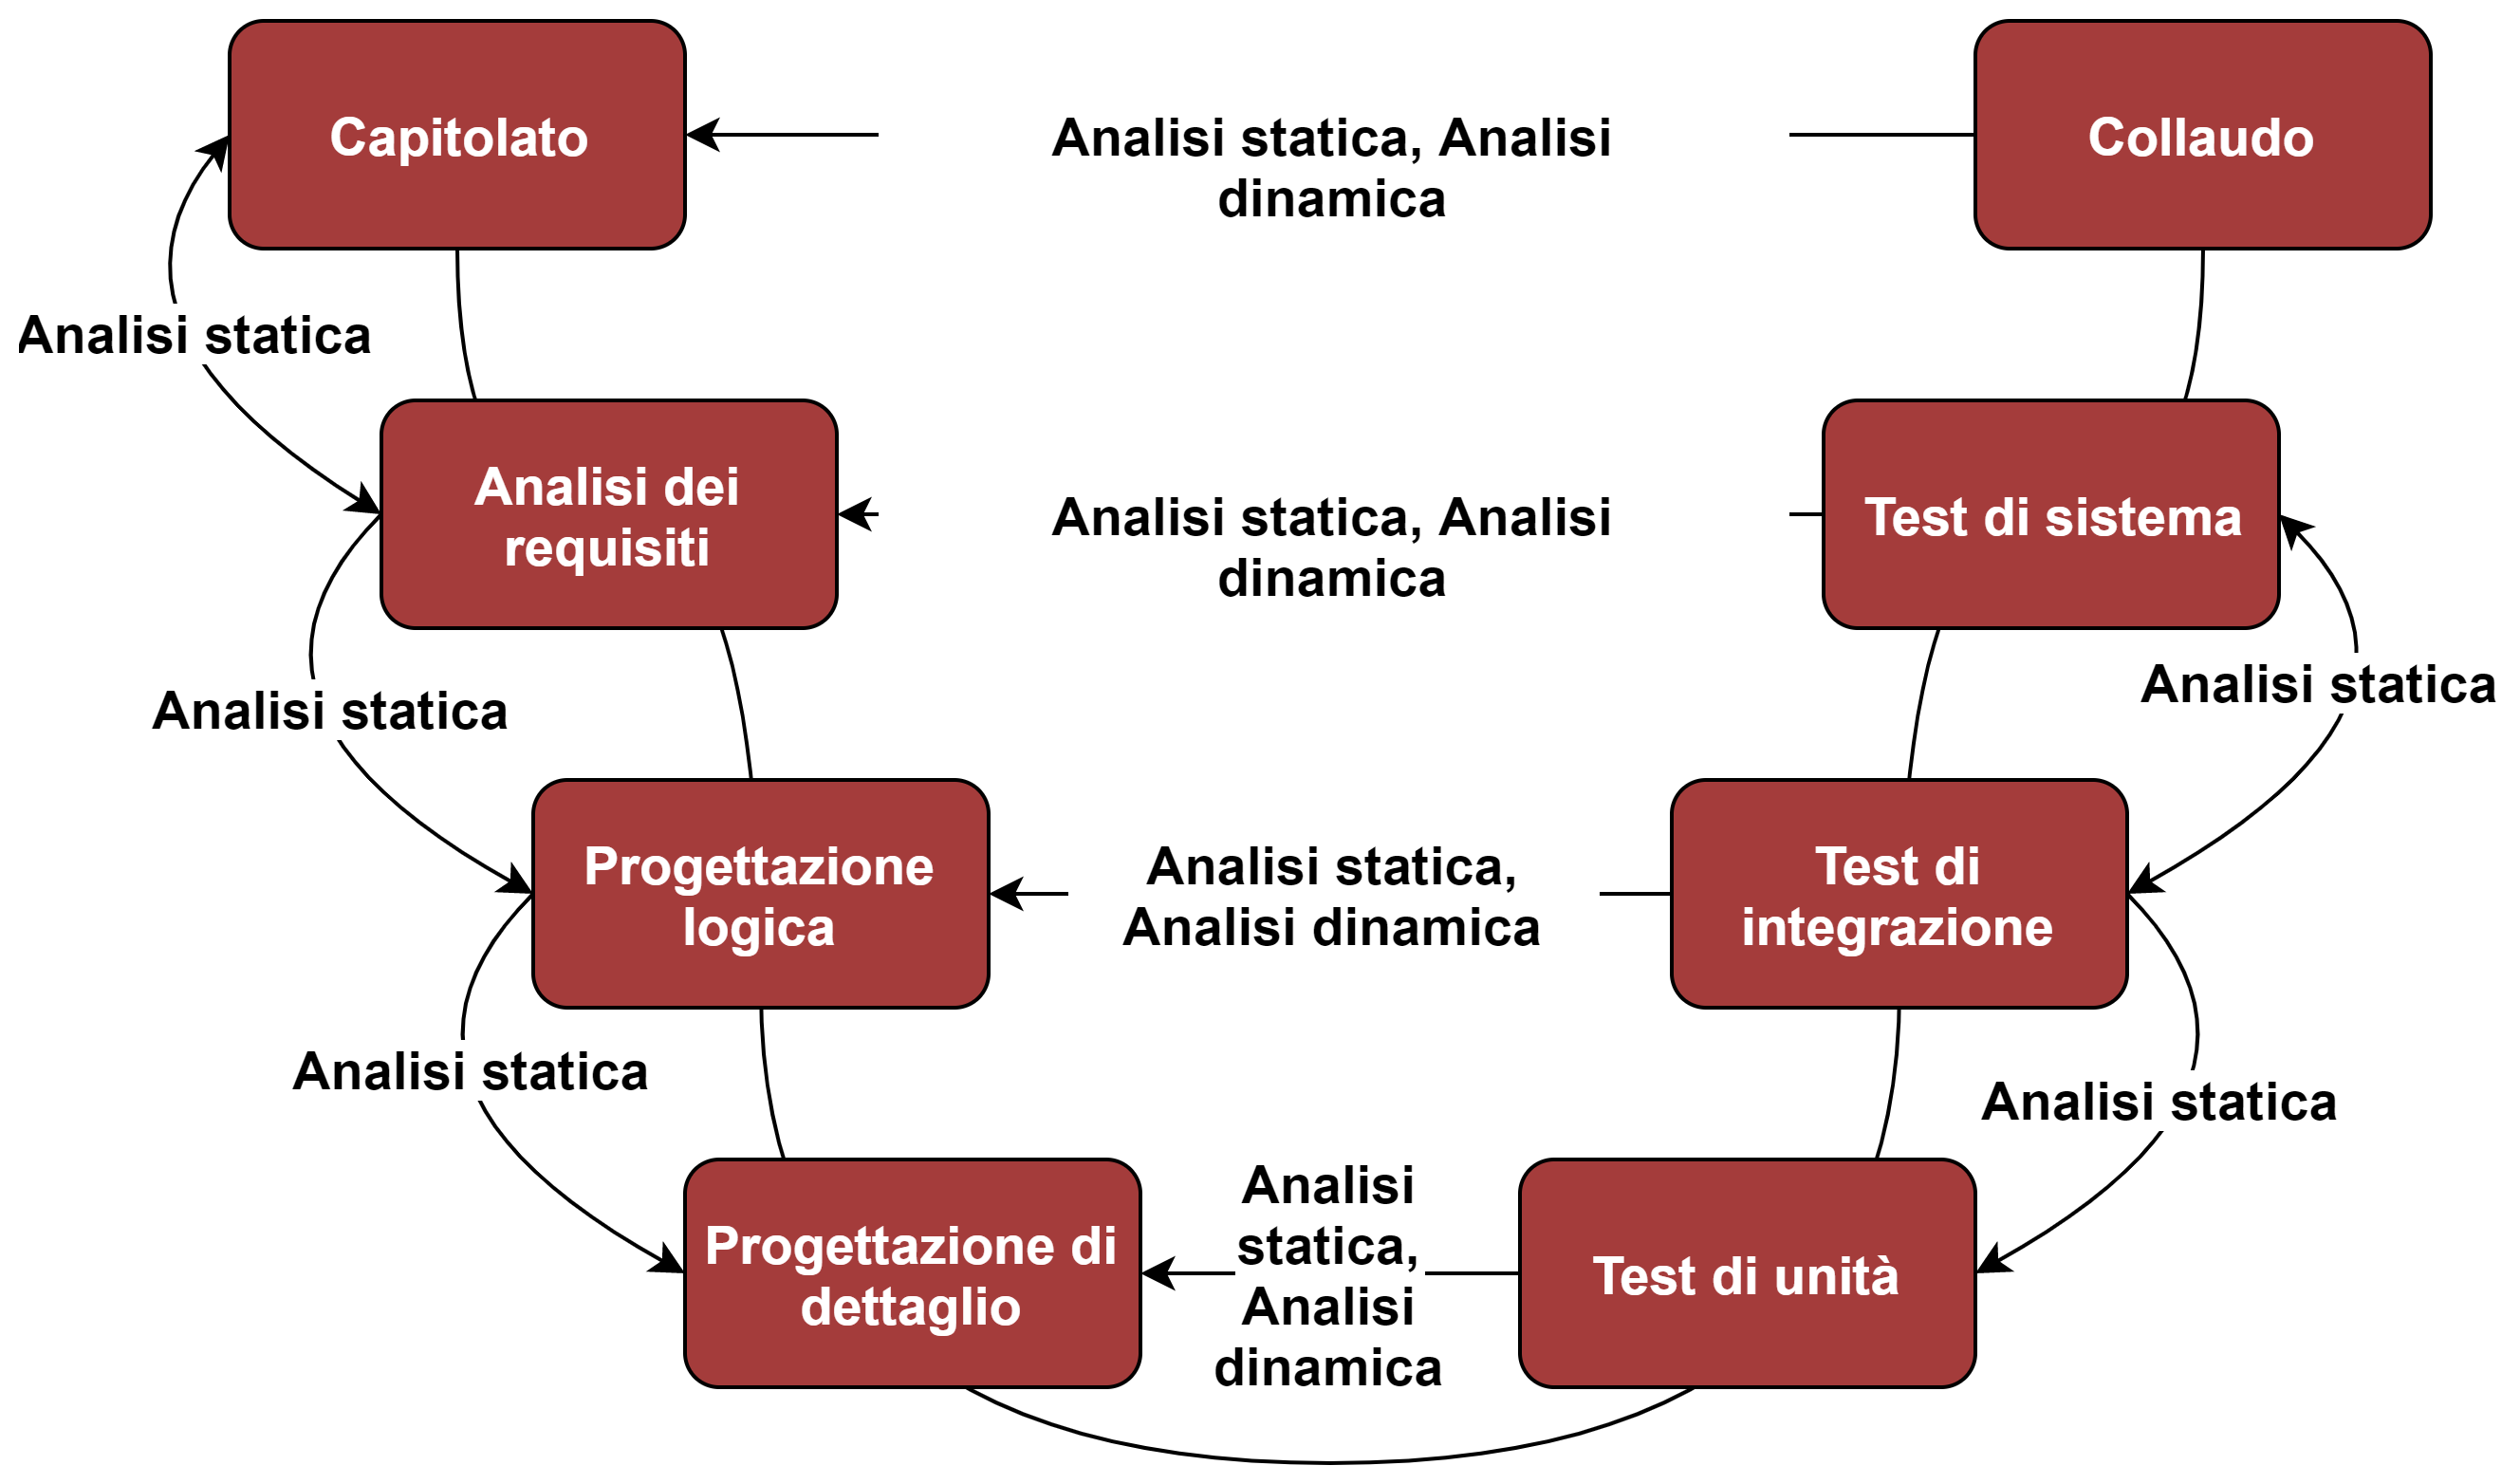
\includegraphics[scale=0.85]{Sezioni/Immagini/ModelloV.png}
    \caption{Modello a V}
\end{figure}

\subsection{Tipologie di test}
I test specificati dal \glo{modello a V} e che devono essere realizzati dal gruppo sono:
\begin{itemize}
    \item \textbf{Test di unità:} Verificano il corretto comportamento di una singola unità del programma. L'unità è una funzionalità atomica verificabile in modo isolato, in modo da assicurare che il risultato dei test su essa non siano influenzati dal comportamento di altre unità; 
    \item \textbf{Test di integrazione:} Verificano il corretto comportamento di più unità che devono cooperare per svolgere appieno i loro compiti;
    \item \textbf{Test di sistema:} Verificano il comportamento dell'intero sistema. I requisiti funzionali, di vincolo, di qualità e di prestazione concordati alla stipulazione del contratto con il committente devono essere soddisfatti per intero;
    \item \textbf{Test di accettazione:} Vengono eseguiti assieme al committente e il loro superamento permette di procedere con il rilascio del prodotto software.
\end{itemize}

\subsubsection{Test di unità}
Allo stato attuale del progetto non è possibile definire quali test di unità dovranno essere realizzati, in quanto devono essere realizzati in contemporanea alla progettazione di dettaglio.\\
Questa sezione del documento verrà redatta non appena inizierà l'attività di progettazione di dettaglio.

{
\rowcolors{2}{grigetto}{white}
\renewcommand{\arraystretch}{1.5}
\centering
\begin{longtable}{ c C{13cm} C{1cm}}
\caption{Elenco dei test di unità}\\
\rowcolor{darkblue}
\textcolor{white}{\textbf{Codice}} & \textcolor{white}{\textbf{Descrizione}} & \textcolor{white}{\textbf{Stato}}\\
\endfirsthead
\rowcolor{darkblue}
\textcolor{white}{\textbf{Codice}} & \textcolor{white}{\textbf{Descrizione}} & \textcolor{white}{\textbf{Stato}}\\
\endhead

TUA1 & Si verifichi che l'utente non \glo{autenticato} possa inserire l'indirizzo e-mail. & NI \\
TUA2 & Si verifichi che l'utente non \glo{autenticato} possa inserire la password. & NI \\
TUA3 & Si verifichi che l'utente non \glo{autenticato} possa ricevere un messaggio di errore se l'\glo{autenticazione} viene negata per inserimento di credenziali errate. & NI \\
TUA4 & Si verifichi che l'utente non \glo{autenticato} possa effettuare il reset della password qualora se la fosse dimenticata. & NI \\
TUA5 & Si verifichi che l’utente non \glo{autenticato} possa inserire l'indirizzo e-mail. & NI \\
TUA6 & Si verifichi che l’utente non \glo{autenticato} possa ricevere un messaggio di errore se tentasse di registrarsi con un'e-mail già usata nel sistema.  & NI \\
TUA7 & Si verifichi che l’utente non \glo{autenticato} possa inserire una password. & NI \\
TUA8 & Si verifichi che l’utente non \glo{autenticato} possa inserire nuovamente la password come conferma. & NI \\
TUA9 & Si verifichi che l’utente non \glo{autenticato} possa ricevere un messaggio di errore qualora abbia inserito una password non ritenuta sicura. Il processo di \glo{autenticazione} deve fallire. & NI \\
TUA10 & Si verifichi che l’utente non \glo{autenticato} possa ricevere un messaggio di errore qualora abbia inserito una conferma password diversa dalla password. Il processo di \glo{autenticazione} deve fallire. & NI \\
TUA11 & Si verifichi che l’utente non \glo{autenticato} possa accettare le condizioni generali d'uso. & NI \\
TUA12 & Si verifichi che la registrazione si interrompa e che l'applicazione si chiuda nel caso che l'utente non autenticato non abbia accettato le condizioni generali d'uso. & NI \\
TUA13 & Si verifichi che l'utente anonimo possa effettuare il \glo{logout} dall'applicazione. & NI \\
TUA14 & Si verifichi che l'utente anonimo possa scaricare la lista di tutte le organizzazioni. & NI \\
TUA15 & Si verifichi che l'utente anonimo riceva un messaggio di errore qualora lo scaricamento della lista di tutte le organizzazioni non vada a buon fine. & NI \\
TUA16 & Si verifichi che l'utente anonimo ossa aggiornare la lista delle organizzazioni tramite \glo{refresh manuale}. & NI \\
TUA17 & Si verifichi che l'utente anonimo possa aggiornare la lista delle organizzazioni tramite \glo{temporizzazione}. & NI \\
TUA18 & Si verifichi che l'utente anonimo possa visionare la lista delle organizzazioni ordinate alfabeticamente. & NI \\
TUA19 & Si verifichi che l'utente anonimo possa visionare la lista delle organizzazioni ordinate secondo la politica \glo{FIFO}. & NI \\
TUA20 & Si verifichi che l'utente anonimo possa visionare la lista delle organizzazioni che permettono il tracciamento anonimo. & NI \\
TUA21 & Si verifichi che l'utente anonimo possa visionare la lista delle organizzazioni che permettono il \glo{tracciamento autenticato}. & NI \\
TUA22 & Si verifichi che l'utente anonimo possa ricercare organizzazioni presenti nella lista delle organizzazioni appartenenti alle nazioni indicate dall'utente. & NI \\
TUA23 & Si verifichi che l'utente anonimo possa ricercare organizzazioni presenti nella lista delle organizzazioni che hanno nel nome una sottostringa scelta dall'utente. & NI \\
TUA24 & Si verifichi che l'utente anonimo possa ricercare organizzazioni presenti nella lista delle organizzazioni appartenenti alla città indicata dall'utente. & NI \\
TUA25 & Si verifichi che l'utente anonimo possa inserire un'organizzazione, presente nella lista di tutte le organizzazioni, nella propria lista delle organizzazioni preferite. & NI \\
TUA26 & Si verifichi che l'utente anonimo possa rimuovere un'organizzazione dalla propria lista delle organizzazioni preferite. & NI \\
TUA27 & Si verifichi che l'utente anonimo venga informato nel caso in cui non sia memorizzata nessuna lista delle organizzazioni del proprio dispositivo. & NI \\
TUA28 & Si verifichi che l'utente riconosciuto possa inserire la modalità di \glo{tracciamento anonimo}. & NI \\
TUA29 & Si verifichi che l'utente riconosciuto possa inserire la modalità di \glo{tracciamento autenticato}. & NI \\
TUA30 & Si verifichi che nel passaggio dalla modalità di \glo{tracciamento autenticato} a quella anonima venga inviata al sistema la richiesta di uscita dell'utente riconosciuto dal luogo e la successiva richiesta di ingresso di utente anonimo. & NI \\
TUA31 & Si verifichi che nel passaggio dalla modalità di \glo{tracciamento anonimo} a quella autenticata venga inviata al sistema la richiesta di uscita dell'utente anonimo dal luogo e la successiva richiesta di ingresso di utente riconosciuto. & NI \\
TUA32 & Si verifichi che l'utente anonimo possa vedere il proprio storico accessi presso un'\glo{organizzazione}. & NI \\
TUA33 & Si verifichi che ogni accesso deve mostrare la data in cui è stato compiuto. & NI \\
TUA34 & Si verifichi che ogni accesso deve mostrare il luogo corrispondente.  & NI \\
TUA35 & Si verifichi che ogni accesso deve mostrare il tempo totale trascorso all'interno nel luogo. & NI \\
TUA36 & Si verifichi che la \glo{lista degli accessi} deve risultare ordinata \glo{per data in ordine decrescente}. & NI \\
TUA37 & Si verifichi che la \glo{lista degli accessi} deve risultare ordinata \glo{per data in ordine crescente}. & NI \\
TUA38 & Si verifichi che nella lista vengono mostrati solo gli accessi che rispettano i parametri di ricerca sul giorno cercato. & NI \\
TUA39 & Si verifichi che l’utente anonimo riceva un messaggio informativo in assenza di accessi effettuati presso un'\glo{organizzazione}. & NI \\
TUA40 & Si verifichi che l’utente anonimo possa visionare il nome dello specifico luogo in cui si trova. & NI \\
TUA41 & Si verifichi che l’utente anonimo possa visionare il tempo trascorso da quando ha fatto l'ultimo ingresso in uno specifico luogo. & NI \\
TUA42 & Si verifichi che l'utente anonimo possa vedere il proprio storico accessi presso il luogo di un'\glo{organizzazione}. & NI \\
TUA43 & Si verifichi che ogni accesso deve mostrare la data in cui è stato compiuto. & NI \\
TUA44 & Si verifichi che ogni accesso deve mostrare il luogo corrispondente. & NI \\
TUA45 & Si verifichi che ogni accesso deve mostrare il tempo totale trascorso all'interno nel luogo. & NI \\
TUA46 & Si verifichi che la \glo{lista degli accessi} deve risultare ordinata \glo{per data in ordine decrescente}. & NI \\
TUA47 & Si verifichi che la \glo{lista degli accessi} deve risultare ordinata \glo{per data in ordine crescente}. & NI \\
TUA48 & Si verifichi che nella lista vengono mostrati solo gli accessi che rispettano i parametri di ricerca sul giorno cercato. & NI \\
TUA49 & Si verifichi che l'utente anonimo, in assenza di accessi effettuati presso il luogo di un'\glo{organizzazione} selezionato, visualizzi un messaggio informativo. & NI \\
TUA50 & Si verifichi che l'utente anonimo possa visualizzare il tempo trascorso all'interno del luogo dall'ultimo ingresso effettuato. & NI \\
TUA51 & Si verifichi che l’utente anonimo riceva la notifica della corretta registrazione se il tracciamento del suo \glo{movimento} in/da un \glo{luogo} ha avuto successo. & NI \\
TUA52 & Si verifichi che l’utente anonimo riceva un messaggio di errore qualora il tracciamento del \glo{movimento} non sia andato a buon fine. & NI \\
TUA53 & Si verifichi che durante la registrazione del \glo{tracciamento} del \glo{movimento} dell'utente anonimo/riconosciuto, venga memorizzato il \glo{timestamp} in cui è avvenuto il \glo{movimento}. & NI \\
TUA54 & Si verifichi che se l'utente riconosciuto è in modalità di \glo{tracciamento autenticato}, venga verificata la correttezza delle credenziali \glo{LDAP}. & NI \\
TUA55 & Si verifichi che se l'utente riconosciuto è in modalità di \glo{tracciamento autenticato}, possa effettuare un ingresso in un luogo dell'\glo{organizzazione}. & NI \\
TUA56 & Si verifichi che se l'utente riconosciuto è in modalità di \glo{tracciamento anonima}, possa effettuare un ingresso in un luogo dell'\glo{organizzazione}. & NI \\
TUA57 & Si verifichi che se l'utente riconosciuto è in modalità di \glo{tracciamento anonima}, possa effettuare un'uscita da un luogo dell'\glo{organizzazione}. & NI \\
TUA58 & Si verifichi che l’utente anonimo possa autenticarsi con credenziali aziendali LDAP in un'organizzazione che richiede il tracciamento riconosciuto. & NI \\
TUA59 & Si verifichi che l’utente anonimo riceva un messaggio di errore qualora le credenziali \glo{LDAP} non fossero riconosciute dal server. & NI \\
TUA60 & Si verifichi che l’utente anonimo possa inserire il proprio nome utente durante l'autenticazione con le credenziali \glo{LDAP} aziendali. & NI \\
TUA61 & Si verifichi che l’utente anonimo possa inserire la propria password utente durante l'autenticazione con le credenziali \glo{LDAP} aziendali. & NI \\
TUS1 & Si verifichi che l’utente non \glo{autenticato} possa inserire l'e-mail correttamente. & NI \\
TUS2 & Si verifichi che l’utente non \glo{autenticato} possa inserire correttamente la password. & NI \\
TUS3 & Si verifichi che l’utente non \glo{autenticato} riceva un messaggio d'errore se l'\glo{autenticazione} viene negata per inserimento di credenziali errate. & NI \\
TUS4 & Si verifichi che l’utente non \glo{autenticato} possa effettuare il reset della password qualora se la fosse dimenticata. & NI \\
TUS5 & Si verifichi che l'amministratore \glo{autenticato} possa effettuare il \glo{logout} dalla applicazione web. & NI \\
TUS6 & Si verifichi che l’amministratore visualizzatore possa selezionare un’organizzazione dalla sua lista delle organizzazioni. & NI \\
TUS7 & Si verifichi che l'amministratore visualizzatore possa visualizzare il nome dell'organizzazione selezionata. & NI \\
TUS8 & Si verifichi che l'amministratore visualizzatore possa visualizzare l’immagine dell'organizzazione selezionata. & NI \\
TUS9 & Si verifichi che l'amministratore visualizzatore possa visualizzare la descrizione dell'organizzazione selezionata. & NI \\
TUS10 & Si verifichi che l'amministratore visualizzatore possa visualizzare l’indirizzo dell'organizzazione selezionata. & NI \\
TUS11 & Si verifichi che l'amministratore visualizzatore possa visualizzare l’indirizzo IP dell'organizzazione selezionata. & NI \\
TUS12 & Si verifichi che l'amministratore visualizzatore possa visualizzare le coordinate geografiche dell'organizzazione selezionata. & NI \\
TUS13 & Si verifichi che l'amministratore gestore possa modificare il nome dell'organizzazione selezionata. & NI \\
TUS14 & Si verifichi che l'amministratore gestore possa modificare l’immagine dell'organizzazione selezionata. & NI \\
TUS15 & Si verifichi che l'amministratore gestore possa modificare la descrizione dell'organizzazione selezionata. & NI \\
TUS16 & Si verifichi che l'amministratore gestore possa modificare l’indirizzo dell'organizzazione selezionata. & NI \\
TUS17 & Si verifichi che l'amministratore gestore possa modificare l’indirizzo IP dell'organizzazione selezionata. & NI \\
TUS18 & Si verifichi che l'amministratore gestore possa modificare le coordinate geografiche dell'organizzazione selezionata. & NI \\
TUS19 & Si verifichi che l'amministratore gestore riceva un messaggio di errore qualora il nome dell'organizzazione inserito non rispetti i vincoli imposti. & NI \\
TUS20 & Si verifichi che l'amministratore gestore possa riceva un messaggio di errore qualora il nome dell'organizzazione inserito sia già presente nel sistema e associato ad un'altra organizzazione. & NI \\
TUS21 & Si verifichi che l'amministratore gestore possa riceva un messaggio di errore qualora l'immagine dell'organizzazione inserita non rispetti i vincoli imposti. & NI \\
TUS22 & Si verifichi che l'amministratore gestore possa riceva un messaggio di errore qualora la descrizione dell'organizzazione inserita non rispetti i vincoli imposti. & NI \\
TUS23 & Si verifichi che l'amministratore gestore possa riceva un messaggio di errore qualora l'indirizzo dell'organizzazione inserito non rispetti i vincoli imposti. & NI \\
TUS24 & Si verifichi che l'amministratore gestore possa riceva un messaggio di errore qualora l'indirizzo IP dell'organizzazione inserito non rappresenti un server \glo{LDAP}. & NI \\
TUS25 & Si verifichi che l'amministratore gestore possa inviare la richiesta di eliminazione per un'organizzazione. & NI \\
TUS26 & Si verifichi che l'amministratore gestore possa inserire una motivazione per la richiesta di eliminazione di un'organizzazione. & NI \\
TUS27 & Si verifichi che l'amministratore gestore possa annullare le modifiche che sta apportando ad una organizzazione. & NI \\
TUS28 & Si verifichi che l’amministratore visualizzatore possa selezionare un luogo di un’organizzazione. & NI \\
TUS29 & Si verifichi che l'amministratore visualizzatore possa visualizzare il nome del luogo di un’organizzazione selezionata. & NI \\
TUS30 & Si verifichi che l'amministratore visualizzatore possa visualizzare le coordinate geografiche del luogo di un’organizzazione selezionata. & NI \\
TUS31 & Si verifichi che l'amministratore gestore possa modificare il nome del luogo di un’organizzazione selezionata. & NI \\
TUS32 & Si verifichi che l'amministratore gestore possa selezionare l'area geografica in cui effettuare il \glo{tracciamento} mediante l'inserimento di coordinate geografiche. & NI \\
TUS33 & Si verifichi che l'amministratore gestore possa selezionare l'area geografica in cui effettuare il \glo{tracciamento} mediante l'inserimento di marcatori su una mappa interattiva. & NI \\
TUS34 & Si verifichi che l'amministratore gestore possa eliminare un luogo di un’organizzazione. & NI \\
TUS35 & Si verifichi che l'amministratore gestore possa annullare le modifiche che sta apportando a un luogo di un’organizzazione.  & NI \\
TUS36 & Si verifichi che l’amministratore visualizzatore possa monitorare il numero degli utenti anonimi all’interno di una organizzazione. & NI \\
TUS37 & Si verifichi che l’amministratore visualizzatore possa monitorare il numero degli utenti anonimi all’interno di un luogo specifico. & NI \\
TUS38 & Si verifichi che l’amministratore visualizzatore possa monitorare gli accessi effettuati da uno specifico utente riconosciuto visualizzandone il nome. & NI \\
TUS39 & Si verifichi che l’amministratore visualizzatore possa monitorare gli accessi effettuati da uno specifico utente riconosciuto visualizzandone il cognome. & NI \\
TUS40 & Si verifichi che l’amministratore visualizzatore possa monitorare gli accessi effettuati da uno specifico utente riconosciuto visualizzandone l’orario di accesso. & NI \\
TUS41 & Si verifichi che l’amministratore visualizzatore possa filtrare la \glo{lista degli accessi} di uno specifico utente riconosciuto per data decrescente. & NI \\
TUS42 & Si verifichi che l’amministratore visualizzatore possa filtrare la \glo{lista degli accessi} di uno specifico utente riconosciuto per data crescente. & NI \\
TUS43 & Si verifichi che l’amministratore visualizzatore possa filtrare la \glo{lista degli accessi} di uno specifico utente riconosciuto per una data precisa. & NI \\
TUS44 & Si verifichi che l’amministratore visualizzatore possa monitorare gli accessi effettuati presso un luogo da uno specifico utente riconosciuto visualizzandone il nome. & NI \\
TUS45 & Si verifichi che l’amministratore visualizzatore possa monitorare gli accessi effettuati presso un luogo da uno specifico utente riconosciuto visualizzandone il cognome. & NI \\
TUS46 & Si verifichi che l’amministratore visualizzatore possa monitorare gli accessi effettuati presso un luogo da uno specifico utente riconosciuto visualizzandone l’orario di accesso. & NI \\
TUS47 & Si verifichi che si possa ottenere un report tabellare degli accesi ai luoghi dell'organizzazione. & NI \\
TUS48 & Si verifichi che si possa generare una tabella contenente il numero degli utenti. & NI \\
TUS49 & Si verifichi che si possa generare una tabella contenente il totale delle ore passate dagli utenti nei luoghi dell’organizzazione. & NI \\
TUS50 & Si verifichi che si possa generare una tabella delle entrate e uscite degli utenti nei luoghi dell'organizzazione. & NI \\
TUS51 & Si verifichi che si possa generare una tabella delle ore spese dagli utenti nei luoghi dell'organizzazione. & NI \\
TUS52 & Si verifichi che l’amministratore proprietario possa visionare gli amministratori che ha precedentemente nominato, di cui si devono visionare la e-mail. & NI \\
TUS53 & Si verifichi che l’amministratore proprietario possa visionare gli amministratori che ha precedentemente nominato, i privilegi. & NI \\
TUS54 & Si verifichi che l’amministratore proprietario possa modificare i privilegi di un altro amministratore, inserendo il suo indirizzo e-mail. & NI \\
TUS55 & Si verifichi che l’amministratore proprietario possa eliminare un amministratore, inserendo il suo indirizzo e-mail. & NI \\
TUS56 & Si verifichi che l’amministratore proprietario riceva un messaggio d'errore se non è presente un amministratore con l'indirizzo e-mail inserito dall'amministratore proprietario. & NI \\
TUS57 & Si verifichi che l’amministratore proprietario possa inserire un nuovo amministratore inserendo l’e-mail. & NI \\
TUS58 & Si verifichi che l’amministratore proprietario possa inserire un nuovo amministratore inserendo la password. & NI \\
TUS59 & Si verifichi che l’amministratore proprietario possa selezionare i privilegi per il nuovo amministratore. & NI \\
TUS60 & Si verifichi che l’amministratore proprietario riceva un messaggio d'errore se l'indirizzo e-mail del nuovo amministratore è già presente nel sistema. & NI \\
TUS61 & Si verifichi che l’amministratore proprietario riceva un messaggio d'errore se la password risulta troppo debole. & NI \\
TUS62 & Si verifichi che l’amministratore proprietario riceva un messaggio d'errore se la conferma della password non combacia con la password. & NI \\
TUS63 & Si verifichi che l’amministratore proprietario possa annullare l'operazione di modifica dei privilegi di un amministratore.  & NI \\
\end{longtable}
}
\newpage
\subsubsection{Tracciamento Requisiti - Test di unità}
{
	\rowcolors{2}{grigetto}{white}
	\renewcommand{\arraystretch}{1.5}
	\centering
	\begin{longtable}{C{2cm} C{12cm}}
		\caption{Tabella di tracciamento requisito-test di unità}\\
		\rowcolor{darkblue}
		\textcolor{white}{\textbf{Codice Test}} & \textcolor{white}{\textbf{Metodo}}\\	
		\endfirsthead
		\rowcolor{darkblue}
		\textcolor{white}{\textbf{Codice Test}} & \textcolor{white}{\textbf{Metodo}}\\	
		\endhead
		TUA1 & LogInFragment::checkLoginDetails()\\
		TUA2 & LogInFragment::checkLoginDetails()\\
		TUA3 & LoginModel::performFirebaseLogin(email:String, password:String)\\
		TUA4 & LoginModel::performResetPassword(email:String)\\
		TUA5 & LoginModel::performResetPassword(email:String)\\
		TUA6 & SignUpModel::performFirebaseRegistration(email:String, password:String)\\
		TUA7 & SignUpFragment::checkSignUpDetails()\\
		TUA8 & SignUpFragment::checkSignUpDetails()\\
		TUA9 & SignUpFragment::checkSignUpDetails()\\
		TUA10 & SignUpFragment::checkSignUpDetails()\\
		TUA11 & SignUpFragment::checkSignUpDetails()\\
		TUA12 & SignUpFragment::checkSignUpDetails()\\
		TUA13 & HomePageActivity::FirebaseAuth.getInstance().signOut()\\
		TUA14 & HomeFragment::downloadList()\\
		TUA15 & HomeFragment::onFailureDownloadList(message:String)\\
		TUA16 & HomeFragment::downloadListWithSwipe()\\
		TUA17 & HomeFragment::downloadListWithSwipe()\\
		TUA18 & HomeFragment::alphabeticalOrder()\\
		TUA19 & HomeFragment::downloadListWithSwipe()\\
		TUA20 & HomeFragment::onOptionsItemSelected (item:MenuItem)\\
		TUA21 & HomeFragment::onOptionsItemSelected (item:MenuItem)\\
		TUA22 & HomeFragment::onOptionsItemSelected (item:MenuItem)\\
		TUA23 & HomeFragment::onQueryTextChange(newText:String)\\
		TUA24 & HomeFragment::onQueryTextChange(newText:String)\\
		TUA25 & FragmentListenerFeatures::addOrganization(Organization organization)\\
		TUA26 & MyStalkerListFragment::removeOrganization(position:int)\\
		TUA27 & MyStalkerListFragment::onFailureLoadMyStalkerList()\\
		TUA28 & HomePageActivity::setSwitchMode()\\
		TUA29 & HomePageActivity::setSwitchMode()\\
		TUA30 & TrackingStalker::performPlaceMovementServer(exitToken:String, type:int, Long:placeID, authID:String, userToken:String, placeAccess:PlaceAccess)\\
		TUA31 & TrackingStalker::performPlaceMovementServer(exitToken:String, type:int, Long:placeID, authID:String, userToken:String, placeAccess:PlaceAccess)\\
		TUA32 & ActionTabFragment::onActivityCreated(Bundle savedInstanceState)\\
		TUA33 & OrganizationAccess::getEntranceTimeStamp()\\
		TUA34 & PlaceAccess::getPlaceName()\\
		TUA35 & OrganizationAccess::getTimeStay()\\
		TUA36 & AccessHistoryFragment::DateDecreasingOrder(list:List<OrganizationAccess>)\\
		TUA37 & AccessHistoryFragment::DateCreasingOrder(list:List<OrganizationAccess>)\\
		TUA38 & AccessHistoryFragment::searchForDay(list:List<OrganizationAccess>)\\
		TUA39 & AccessHistoryFragment::onFailureGetOrganizationAccessInLocal()\\
		TUA40 & HomePageActivity::getNamePlace()\\
		TUA41 & PlaceAccess::getTimeStay()\\
		TUA42 & PlaceAccessFragment::onSuccessGetPlaceAccessInLocal(placeAccessList:List<PlaceAccess>)\\
		TUA43 & PlaceAccess::getDate()\\
		TUA44 & PlaceAccessFragment::onSuccessGetPlaceAccessInLocal(placeAccessList:List<PlaceAccess>)\\
		TUA45 & PlaceAccess::getTimeStay()\\
		TUA46 & AccessHistoryFragment::DateDecreasingOrder(list:List<OrganizationAccess>)\\
		TUA47 & AccessHistoryFragment::DateCreasingOrder(list:List<OrganizationAccess>)\\
		TUA48 & AccessHistoryFragment::searchForDay(list:List<OrganizationAccess>)\\
		TUA49 & AccessHistoryFragment::onFailureGetOrganizationAccessInLocal()\\
		TUA50 & PlaceAccess::getTimeStay()\\
		TUA51 & TrackingStalker::isInsidePlace(location:Location)\\
		TUA52 & Server::performOrganizationMovementServer(authID:String, orgID:Long, userToken:String, type:int, exitToken:String, orgAccess:OrganizationAccess)\\
		TUA53 & TrackingStalker::isInsideOrganization(location:Location)\\
		TUA54 & Server::performOrganizationMovementServer(authID:String, orgID:Long, userToken:String, type:int, exitToken:String, orgAccess:OrganizationAccess)\\
		TUA55 & TrackingStalker::isInsidePlace(location:Location)\\
		TUA56 & TrackingStalker::isInsidePlace(location:Location)\\
		TUA57 & TrackingStalker::isInsidePlace(location:Location)\\
		TUA58 & StalkerLDAP::performBind()\\
		TUA59 & StalkerLDAP::performSearch()\\
		TUA60 & StalkerLDAP::getBindDN()\\
		TUA61 & StalkerLDAP::getBindPassword()\\
		TUB1 & AccessApiController::getAnonymousAccessListInOrganization()\\
		TUB2 & AccessApiController::getAnonymousAccessListInOrganization()\\
		TUB3 & AccessApiController::getAnonymousAccessListInPlace()\\
		TUB4 & AccessApiController::getAnonymousAccessListInPlace()\\
		TUB5 & AccessApiController::getAuthenticatedAccessListInOrganization()\\
		TUB6 & AccessApiController::getAuthenticatedAccessListInOrganization()\\
		TUB7 & AccessApiController::getAuthenticatedAccessListInPlace()\\
		TUB8 & AccessApiController::getAuthenticatedAccessListInPlace()\\
		TUB9 & AdministratorApiController::bindAdministratorToOrganization()\\
		TUB10 & AdministratorApiController::bindAdministratorToOrganization()\\
		TUB11 & AdministratorApiController::createNewAdministratorInOrganization()\\
		TUB12 & AdministratorApiController::createNewAdministratorInOrganization()\\
		TUB13 & AdministratorApiController::getAdministratorListOfOrganization()\\
		TUB14 & AdministratorApiController::getAdministratorListOfOrganization()\\
		TUB15 & AdministratorApiController::getPermissionList()\\
		TUB16 & AdministratorApiController::getPermissionList()\\
		TUB17 & AdministratorApiController::unbindAdministratorFromOrganization()\\
		TUB18 & AdministratorApiController::unbindAdministratorFromOrganization()\\
		TUB19 & AdministratorApiController::updateAdministratorPermission()\\
		TUB20 & AdministratorApiController::updateAdministratorPermission()\\
		TUB21 & FavoriteApiController::addFavoriteOrganization()\\
		TUB22 & FavoriteApiController::addFavoriteOrganization()\\
		TUB23 & FavoriteApiController::getFavoriteOrganizationList()\\
		TUB24 & FavoriteApiController::getFavoriteOrganizationList()\\
		TUB25 & FavoriteApiController::removeFavoriteOrganization()\\
		TUB26 & FavoriteApiController::removeFavoriteOrganization()\\
		TUB27 & MovementApiController::trackMovementInOrganization()\\
		TUB28 & MovementApiController::trackMovementInOrganization()\\
		TUB29 & MovementApiController::trackMovementInPlace()\\
		TUB30 & MovementApiController::trackMovementInPlace()\\
		TUB31 & OrganizationApiController::getOrganization()\\
		TUB32 & OrganizationApiController::getOrganization()\\
		TUB33 & OrganizationApiController::getOrganizationList()\\
		TUB34 & OrganizationApiController::getOrganizationList()\\
		TUB35 & OrganizationApiController::requestDeletionOfOrganization()\\
		TUB36 & OrganizationApiController::requestDeletionOfOrganization()\\
		TUB37 & OrganizationApiController::updateOrganization()\\
		TUB38 & OrganizationApiController::updateOrganization()\\
		TUB39 & OrganizationApiController::updateOrganizationTrackingArea()\\
		TUB40 & OrganizationApiController::updateOrganizationTrackingArea()\\
		TUB41 & PlaceApiController::createNewPlace()\\
		TUB42 & PlaceApiController::createNewPlace()\\
		TUB43 & PlaceApiController::deletePlace()\\
		TUB44 & PlaceApiController::deletePlace()\\
		TUB45 & PlaceApiController::updatePlace()\\
		TUB46 & PlaceApiController::updatePlace()\\
		TUB47 & PlaceApiController::getPlaceListOfOrganization()\\
		TUB48 & PlaceApiController::getPlaceListOfOrganization()\\
		TUB49 & PresenceApiController::getOrganizationPresenceCounter()\\
		TUB50 & PresenceApiController::getOrganizationPresenceCounter()\\
		TUB51 & PresenceApiController::getPlacePresenceCounter()\\
		TUB52 & PresenceApiController::getPlacePresenceCounter()\\
		TUB53 & ReportApiController::getTimePerUserReport()\\
		TUB54 & ReportApiController::getTimePerUserReport()\\
		TUB55 & AdministratorServiceImpl::bindAdministratorToOrganization()\\
		TUB56 & AdministratorServiceImpl::bindAdministratorToOrganization()\\
		TUB57 & AdministratorServiceImpl::bindAdministratorToOrganization()\\
		TUB58 & AdministratorServiceImpl::createNewAdministratorInOrganization()\\
		TUB59 & AdministratorServiceImpl::createNewAdministratorInOrganization()\\
		TUB60 & AdministratorServiceImpl::getAdministratorListOfOrganization()\\
		TUB61 & AdministratorServiceImpl::getPermissionList()\\
		TUB62 & AdministratorServiceImpl::updateAdministratorPermission()\\
		TUB63 & AdministratorServiceImpl::updateAdministratorPermission()\\
		TUB64 & AdministratorServiceImpl::unbindAdministratorFromOrganization()\\
		TUB65 & AccessServiceImpl::getAnonymousAccessListInOrganization()\\
		TUB66 & AccessServiceImpl::getAnonymousAccessListInOrganization()\\
		TUB67 & AccessServiceImpl::getAnonymousAccessListInPlace()\\
		TUB68 & AccessServiceImpl::getAnonymousAccessListInPlace()\\
		TUB69 & AccessServiceImpl::getAuthenticatedAccessListInOrganization()\\
		TUB70 & AccessServiceImpl::getAuthenticatedAccessListInOrganization()\\
		TUB71 & AccessServiceImpl::getAuthenticatedAccessListInPlace()\\
		TUB72 & AccessServiceImpl::getAuthenticatedAccessListInPlace()\\
		TUB73 & AuthenticationServiceImpl::isWebAppAdministrator()\\
		TUB74 & AuthenticationServiceImpl::isWebAppAdministrator()\\
		TUB75 & AuthenticationServiceImpl::isWebAppAdministrator()\\
		TUB76 & AuthenticationServiceImpl::isAppUser()\\
		TUB77 & AuthenticationServiceImpl::isAppUser()\\
		TUB78 & AuthenticationServiceImpl::isAppUser()\\
		TUB79 & AuthenticationServiceImpl::createUser()\\
		TUB80 & AuthenticationServiceImpl::createUser()\\
		TUB81 & AuthenticationServiceImpl::createUser()\\
		TUB82 & AuthenticationServiceImpl::createUser()\\
		TUB83 & AuthenticationServiceImpl::createUser()\\
		TUB84 & AuthenticationServiceImpl::createUser()\\
		TUB85 & AuthenticationServiceImpl::createUser()\\
		TUB86 & AuthenticationServiceImpl::getUserIdByEmail()\\
		TUB87 & AuthenticationServiceImpl::getUserIdByEmail()\\
		TUB88 & AuthenticationServiceImpl::getUserIdByEmail()\\
		TUB89 & AuthenticationServiceImpl::getUserIdByEmail()\\
		TUB90 & AuthenticationServiceImpl::getUserIdByEmail()\\
		TUB91 & AuthenticationServiceImpl::getUserIdByEmail()\\
		TUB92 & AuthenticationServiceImpl::getUserId()\\
		TUB93 & AuthenticationServiceImpl::getUserId()\\
		TUB94 & AuthenticationServiceImpl::getFirebaseUser()\\
		TUB95 & AuthenticationServiceImpl::getFirebaseUser()\\
		TUB96 & FavoriteServiceImpl::addFavoriteOrganization()\\
		TUB97 & FavoriteServiceImpl::addFavoriteOrganization()\\
		TUB98 & FavoriteServiceImpl::getFavoriteOrganizationList()\\
		TUB99 & FavoriteServiceImpl::removeFavoriteOrganization()\\
		TUB100 & FavoriteServiceImpl::getFavorite()\\
		TUB101 & FavoriteServiceImpl::getFavorite()\\
		TUB102 & PresenceServiceImpl::getOrganizationPresenceCounter()\\
		TUB103 & PresenceServiceImpl::getPlacePresenceCounter()\\
		TUB104 & MovementServiceImpl::trackMovementInOrganization()\\
		TUB105 & MovementServiceImpl::trackMovementInOrganization()\\
		TUB106 & MovementServiceImpl::trackMovementInOrganization()\\
		TUB107 & MovementServiceImpl::trackMovementInOrganization()\\
		TUB108 & MovementServiceImpl::trackMovementInOrganization()\\
		TUB109 & MovementServiceImpl::trackMovementInPlace()\\
		TUB110 & MovementServiceImpl::trackMovementInPlace()\\
		TUB111 & MovementServiceImpl::trackMovementInPlace()\\
		TUB112 & MovementServiceImpl::trackMovementInPlace()\\
		TUB113 & MovementServiceImpl::trackMovementInPlace()\\
		TUB114 & ReportServiceImpl::getTimePerUserReport()\\
		TUB115 & ReportServiceImpl::getTimePerUserReport()\\
		TUB116 & OrganizationServiceImpl::getOrganization()\\
		TUB117 & OrganizationServiceImpl::getOrganization()\\
		TUB118 & OrganizationServiceImpl::getOrganizationList()\\
		TUB119 & OrganizationServiceImpl::getOrganizationList()\\
		TUB120 & OrganizationServiceImpl::updateOrganization()\\
		TUB121 & OrganizationServiceImpl::updateOrganization()\\
		TUB122 & OrganizationServiceImpl::updateOrganizationTrackingArea()\\
		TUB123 & OrganizationServiceImpl::updateOrganizationTrackingArea()\\
		TUB124 & PlaceServiceImpl::createNewPlace()\\
		TUB125 & PlaceServiceImpl::deletePlace()\\
		TUB126 & PlaceServiceImpl::updatePlace()\\
		TUB127 & PlaceServiceImpl::updatePlace()\\
		TUB128 & PlaceServiceImpl::getPlace()\\
		TUB129 & PlaceServiceImpl::getPlace()\\
		TUW1 & LoginComponent::createForm() \\
		TUW2 & LoginComponent::createForm() \\
		TUW3 & AuthenticationService::SignWithEmailPassword() \\
		TUW4 & AuthenticationService::ResetPassword() \\
		TUW5 & AuthenticationService::SignOut() \\
		TUW6 & MenuBarComponent::SetOrganization() \\
		TUW7 & OrganizationInformationContentComponent::getName() \\
		TUW8 & OrganizationInformationContentComponent::getImg() \\
		TUW9 & OrganizationInformationContentComponent::getDesc() \\
		TUW10 & OrganizationInformationContentComponent::getInd() \\
		TUW11 & OrganizationInformationContentComponent::getLDAP() \\
		TUW12 & ViewOrganizationTrackingAreaContentComponent::receiveMap() \\
		TUW13 & OrganizationManagementContentComponent::setName() \\
		TUW14 & OrganizationManagementContentComponent::setImg() \\
		TUW15 & OrganizationManagementContentComponent::setDescr() \\
		TUW16 & OrganizationManagementContentComponent::setInd() \\
		TUW17 & OrganizationManagementContentComponent::setLDAP() \\
		TUW18 & ModifyOrganizationTrackingAreaContentComponent::OnModify() \\
		TUW19 & OrganizationManagementContentComponent::OnModify() \\
		TUW20 & OrganizationManagementContentComponent::OnModify() \\
		TUW21 & OrganizationManagementContentComponent::OnModify() \\
		TUW22 & OrganizationManagementContentComponent::OnModify() \\
		TUW23 & OrganizationManagementContentComponent::OnModify() \\
		TUW24 & OrganizationManagementContentComponent::OnModify() \\
		TUW25 & OrganizationManagementContentComponent::OnRemove() \\
		TUW26 & OrganizationManagementContentComponent::OnRemove() \\
		TUW27 & OrganizationManagementContentComponent::Reset() \\
		TUW28 & AdministratorOrganizationDataService::setCurrentOrganizationPlaces()\\
		TUW29 & PlaceManagementContentComponent::getName() \\
		TUW30 & ViewOrganizationTrackingAreaContentComponent::receiveMap() \\
		TUW31 & PlaceManagementContentComponent::setName() \\
		TUW32 & ModifyPlaceTrackingAreaContentComponent::OnModify() \\
		TUW33 & ModifyPlaceTrackingAreaContentComponent::OnModify() \\
		TUW34 & PlaceManagementContentComponent::OnRemove() \\
		TUW35 & PlaceManagementContentComponent::Reset() \\
		TUW36 & OrganizationPresenceNumberComponent::subscribeToCounter() \\
		TUW37 & PlacePresenceNumberComponent::subscribeToCounter() \\
		TUW38 & AuthenticatedUserAccessesComponent::getName() \\
		TUW39 & AuthenticatedUserAccessesComponent::getSurname() \\
		TUW40 & AuthenticatedUserAccessesComponent::getEntranceTimestamp() \\
		TUW41 & AuthenticatedUserAccessesComponent::sortEnterOrgAccesses(mode: number) \\
		TUW42 & AuthenticatedUserAccessesComponent::sortEnterOrgAccesses(mode: number) \\
		TUW43 & AuthenticatedUserAccessesComponent::sortByDay() \\
		TUW44 & AuthenticatedUserAccessesComponent::getName() \\
		TUW45 & AuthenticatedUserAccessesComponent::getSurname() \\
		TUW46 & AuthenticatedUserAccessesComponent::getEntranceTimestamp() \\
		TUW47 & TimeReportComponent::timeSpentBy(placeArrIndex: number, ordID: string) \\
		TUW48 & TimeReportComponent::getNumberUser() \\
		TUW49 & TimeReportComponent::timeSpentBy(placeArrIndex: number, ordID: string) \\
		TUW50 & AuthenticatedUserAccessesComponent::ViewAccess() \\
		TUW51 & TimeReportComponent::timeSpentBy(placeArrIndex: number, ordID: string) \\
		TUW52 & AdministratorManagementComponent::getMail() \\
		TUW53 & AdministratorManagementComponent::getPermission() \\
		TUW54 & AdministratorManagementComponent::modifyPermissionsOf() \\
		TUW55 & AdministratorManagementComponent::unbindAdminFromTheOrganization() \\
		TUW56 & AdministratorManagementComponent::checkEmail() \\
		TUW57 & AdministratorManagementComponent::SetupForm() \\
		TUW58 & AdministratorManagementComponent::SetupForm() \\
		TUW59 & AdministratorManagementComponent::SetPermission() \\
		TUW60 & CreateAdministratorComponent::registerAdministrator() \\
		TUW61 & CreateAdministratorComponent::registerAdministrator() \\
		TUW62 & CreateAdministratorComponent::checkPsw() \\
		TUW63 & CreateAdministratorComponent::Reset() \\
		
	\end{longtable}
}
\newpage

\subsubsection{Test di integrazione}
Allo stato attuale del progetto non è possibile definire quali test di integrazione dovranno essere realizzati, in quanto devono essere realizzati in contemporanea alla progettazione di dettaglio.\\
Questa sezione del documento verrà redatta non appena inizierà l'attività di progettazione di dettaglio.

{
\rowcolors{2}{grigetto}{white}
\renewcommand{\arraystretch}{1.5}
\centering
\begin{longtable}{ c  C{8.5cm} C{3cm}}
\caption{Elenco dei test di unità}\\
\rowcolor{darkblue}
\textcolor{white}{\textbf{Codice}} & \textcolor{white}{\textbf{Descrizione}} & \textcolor{white}{\textbf{Stato}}\\
\endfirsthead
\rowcolor{darkblue}
\textcolor{white}{\textbf{Codice}} & \textcolor{white}{\textbf{Descrizione}} & \textcolor{white}{\textbf{Stato}}\\
\endhead

TI1 & ??? & ??? \\

\end{longtable}
}
\newpage
\subsection{Tracciamento Requisiti - Test di Integrazione}
{
	\rowcolors{2}{grigetto}{white}
	\renewcommand{\arraystretch}{1.5}
	\centering
	\begin{longtable}{C{2cm} C{12cm}}
	\caption{Tabella di tracciamento requisito-test di integrazione}\\
	\rowcolor{darkblue}
	\textcolor{white}{\textbf{Codice Test}} & \textcolor{white}{\textbf{Metodo}}\\	
	\endfirsthead
	\rowcolor{darkblue}
	\textcolor{white}{\textbf{Codice Test}} & \textcolor{white}{\textbf{Metodo}}\\	
	\endhead
	
	TIA1 &  \\
	TIA2 &  \\
	TIA3 &  \\
	TIA4 &  \\
	TIA5 &  \\
	TIA6 &  \\
	TIA7 &  \\
	TIA8 &  \\
	TIA9 &  \\
	TIA10 &  \\
	TIA11 &  \\
	TIA12 &  \\
	TIA13 &  \\
	TIA14 &  \\
	TIA15 &  \\
	TIA16 &  \\
	TIA17 &  \\
	TIA18 &  \\
	TIA19 &  \\
	TIA20 &  \\
	TIB1 & GET /administrator/organization/\{organizationId\} \\
	TIB2 & POST /favorite/removefavorite \\
	TIB3 & GET /administrator/organization/\{organizationId\} \\
	TIB4 & POST /favorite/removefavorite \\
	TIB5 & GET /organization/\{organizationId\} \\
	TIB6 & GET /place/organization/\{organizationId\} \\
	TIB7 & POST /administrator/createadministrator \\
	TIB8 & POST /administrator/bindadministrator \\
	TIB9 & POST /administrator/unbindadministrator \\
	TIB10 & GET /administrator/permission/\{administratorId\} \\
	TIB11 & POST /favorite/addfavorite \\
	TIB12 & POST /favorite/removefavorite \\
	TIB13 & POST /movement/track/organization \\
	TIB14 & POST /movement/track/place \\
	TIB15 & PUT /organization \\
	TIB16 & POST /place \\
	TIB17 & PUT /place \\
	TIB18 & PATCH /administrator/updatepermission \\
	TIB19 & POST /administrator/createadministrator \\
	TIB20 & PATCH /administrator/updatepermission \\
	TIB21 & POST /favorite/addfavorite \\
	TIB22 & GET /favorite/\{userId\} \\
	TIB23 & POST /movement/track/organization \\
	TIB24 & PATCH /organization/\{organizationId\}/trackingArea \\
	TIB25 & GET /presence/organization/\{organizationId\}/counter \\
	TIB26 & GET /presence/place/\{placeId\}/counter \\
	TIB27 & GET /access/organization/\{organizationId\}/authenticated/\{orgAuthServerIds\} \\
	TIB28 & GET /access/place/\{placeId\}/authenticated/\{orgAuthServerIds\} \\
	TIB29 & GET /administrator/organization/\{organizationId\} \\
	TIB30 & GET /administrator/permission/\{administratorId\} \\
	TIB31 & GET /favorite/\{userId\} \\
	TIB32 & GET /organization/\{organizationId\} \\
	TIB33 & GET /organization/\{organizationId\} \\
	TIB34 & PUT /organization \\
	TIB35 & PATCH /organization/\{organizationId\}/trackingArea \\
	TIB36 & GET /place/organization/\{organizationId\} \\
	TIB37 & PUT /place \\
	TIB38 & GET /presence/organization/\{organizationId\}/counter \\
	TIB39 & GET /presence/place/\{placeId\}/counter \\
	TIB40 & GET /report/place/\{placeId\} \\
	TIB41 & POST /administrator/bindadministrator \\
	TIB42 & POST /administrator/bindadministrator \\
	TIB43 & PATCH /administrator/updatepermission \\
	TIB44 & POST /favorite/addfavorite \\
	TIB45 & POST /movement/track/organization \\
	TIB46 & POST /movement/track/place \\
	TIB47 & POST /place \\
	TIB48 & POST /movement/track/organization \\
	TIB49 & POST /movement/track/place \\
	TIB50 & POST /movement/track/organization \\
	TIB51 & POST /movement/track/place \\
	TIB52 & GET /access/organization/\{organizationId\}/authenticated/\{orgAuthServerIds\} \\
	TIB53 & GET /access/place/\{placeId\}/authenticated/\{orgAuthServerIds\} \\
	TIB54 & GET /favorite/\{userId\} \\
	TIB55 & GET /organization \\
	TIB56 & GET /place/organization/\{organizationId\} \\
	TIB57 & PUT /place \\
	TIB58 & GET /report/place/\{placeId\} \\
	TIB59 & POST /organization/requestdeletion \\
	TIB60 & POST /administrator/unbindadministrator \\
	TIB61 & POST /favorite/removefavorite \\
	TIB62 & DELETE /place/\{placeId\} \\
	TIW1 & Authentication::signInWithEmailAndPassword(email:string,psw:string) \\
	TIW2 & Authentication::sendPasswordResetEmail(email:string) \\
	TIW3 & Authentication::authState()\\
	TIW4 & AuthenticationServerService::getUserInfoFromAuthServer(organizationAuthenticationServerRequest: OrganizationAuthenticationServerRequest) \\
	TIW5 & GeneralService::constructor(protected httpClient: HttpClient, basePath: string, configuration: Configuration) \\
	TIW6 & AdministratorService::getPermissionList(administratorId: string)\\
	TIW7 & AdministratorService:: getListOrganization(administratorId: string)\\
	TIW8 & PlaceService::getPlaceListOfOrganization(organizationId: number)\\
	TIW9 & PresenceService::getOrganizationPresenceCounter(organizationId: number)\\
	TIW10 & PresenceService::getPlacePresenceCounter(organizationId: number)\\
	TIW11 & OrganizationService::getOrganization(organizationId: number)\\
	TIW12 & PlaceService::getPlaceListOfOrganization(organizationId: number)\\
	TIW13 & OrganizationService::updateOrganization(organization: Organization)\\
	TIW14 & PlaceService::updatePlace(place: Place)\\
	TIW15 & PlaceService::createNewPlace(place: Place)\\
	TIW16 & AdministratorService::createNewAdministratorInOrganization(administratorBindingRequest: AdministratorBindingRequest)\\
	TIW17 & OrganizationService::requestDeletionOfOrganization(organizationDeletionRequest: OrganizationDeletionRequest)\\
	TIW18 & PlaceService::deletePlace(placeId: number)\\
	TIW19 & AdministratorService::updateAdministratorPermission(permission: Permission)\\
	TIW20 & AdministratorService::unbindAdministratorFromOrganization(permission: Permission)\\


\end{longtable}
}
\newpage

\subsubsection{Test di sistema}
I test di sistema devono assicurare la completa copertura dei requisiti espressi nel documento \AdR{}.
Segue l'elenco dei test di sistema con la relativa descrizione.

{
\rowcolors{2}{grigetto}{white}
\renewcommand{\arraystretch}{1.5}
\centering
\begin{longtable}{ c  C{2.5cm}  C{10cm} C{1cm}}
\caption{Elenco dei test di sistema}\\
\rowcolor{darkblue}
\textcolor{white}{\textbf{Codice}} & \textcolor{white}{\textbf{Titolo}} & \textcolor{white}{\textbf{Descrizione}} & \textcolor{white}{\textbf{Stato}}\\
\endfirsthead
\rowcolor{darkblue}
\textcolor{white}{\textbf{Codice}} & \textcolor{white}{\textbf{Titolo}} & \textcolor{white}{\textbf{Descrizione}} & \textcolor{white}{\textbf{Stato}}\\
\endhead

%da R1FI1 a R1FA8.4 (con parti splittate) % Christian
TSA1 & Accesso all'applicazione di un utente non autenticato con credenziali Stalker &
Verificare che l'utente non autenticato:
\begin{enumerate}
    \item Possa inserire l'indirizzo e-mail;
    \item Possa inserire la password;
    \item Riceva un messaggio di errore se l'\glo{autenticazione} viene negata per inserimento di credenziali errate.
\end{enumerate}
Se l'utente non autenticato si è dimenticato la sua password:
\begin{enumerate}[resume]
    \item Verifica che l'utente non autenticato possa effettuare il reset della password qualora se la fosse dimenticata.
\end{enumerate} & ?? \\

%da R1FI1 a R1FA8.4 (con parti splittate) % Christian
TSA2 & Registrazione nell'applicazione di un utente non autenticato con credenziali Stalker &
Verificare che l'utente non autenticato:
\begin{enumerate}
    \item Possa inserire l'indirizzo e-mail;
    \item Riceva un messaggio di errore se tentasse di registrarsi con un'e-mail già usata nel sistema;
    \item Possa inserire una password;
    \item Possa inserire nuovamente la password come conferma;
    \item Riceva un messaggio di errore qualora abbia inserito una password non ritenuta sicura. Il processo di \glo{autenticazione} deve fallire;
    \item Riceva un messaggio di errore qualora abbia inserito una conferma password diversa dalla password. Il processo di \glo{autenticazione} deve fallire;
    \item Possa accettare le condizioni generali d'uso;
    \item La registrazione si interrompa e che l'applicazione si chiuda nel caso che l'utente non autenticato non abbia accettato le condizioni generali d'uso.
\end{enumerate} & ?? \\

% R1FA2.1
TSA3  & \glo{Logout} dell'utente anonimo & \begin{enumerate}
    \item Verifica che l'utente anonimo possa effettuare il \glo{logout} dall'applicazione.
\end{enumerate} & ?? \\

% da R1FA3.1, R1FA3.2, R1FA8.5, R1FA3.7, R1FA3.8, R1FA3.9 % Riccardo
TSA4 & Gestione lista delle \glo{organizzazioni} &
Verificare che l'utente anonimo:
\begin{enumerate}
    \item Possa scaricare la lista di tutte le organizzazioni;
    \item Riceva un messaggio di errore qualora lo scaricamento della lista di tutte le organizzazioni non vada a buon fine;
    \item Possa aggiornare la lista delle organizzazioni tramite \glo{refresh manuale};
    \item Possa aggiornare la lista delle organizzazioni tramite \glo{temporizzazione}.
\end{enumerate} & ?? \\

% R1FA3.10, R1FA3.11, R1FA3.12, R1FA3.13, R1FA3.14, R1FA3.15, R1FA3.16, R1FA3.17, R1FA3.18 % Riccardo
TSA5 & Visualizzazione lista delle organizzazioni & 
Verificare che l'utente anonimo:
\begin{enumerate}
% \item Possa autenticarsi con credenziali LDAP, qualora scaricasse una organizzazione che richieda l'autenticazione con credenziali LDAP;
    \item Possa visionare la lista delle organizzazioni ordinate alfabeticamente;
    \item Possa visionare la lista delle organizzazioni ordinate secondo la politica \glo{FIFO};
    \item Possa visionare la lista delle organizzazioni che permettono il tracciamento anonimo;
    \item Possa visionare la lista delle organizzazioni che permettono il \glo{tracciamento autenticato};
    \item Possa ricercare organizzazioni presenti nella lista delle organizzazioni appartenenti alle nazioni indicate dall'utente;
    \item Possa ricercare organizzazioni presenti nella lista delle organizzazioni che hanno nel nome una sotto-stringa scelta dall'utente;
    \item Possa ricercare organizzazioni presenti nella lista delle organizzazioni appartenenti alla città indicata dall'utente.
\end{enumerate} & ?? \\

% da R1FA3.3, R1FA3.4, R1FA3.5, R1FA3.6, R1FA8.6 % Riccardo
TSA6 & Gestione lista delle organizzazioni preferite dell'utente anonimo &
Verificare che l'utente anonimo:
\begin{enumerate}
    \item Possa inserire un'organizzazione, presente nella lista di tutte le organizzazioni, nella propria lista delle organizzazioni preferite;
    \item Possa rimuovere un'organizzazione dalla propria lista delle organizzazioni preferite;
    \item Venga informato nel caso in cui non sia memorizzata nessuna lista delle organizzazioni del proprio dispositivo.
\end{enumerate} & ?? \\

% da R1FA4.1 a R1FA4.3 % Tommaso
TSA7 & Selezione della modalità di \glo{tracciamento} & 
\glo{Verificare} che l'utente riconosciuto:
\begin{enumerate}
    \item Possa inserire la modalità di \glo{tracciamento anonimo};
    \item Possa inserire la modalità di \glo{tracciamento autenticato}.
\end{enumerate}
Se l'utente riconosciuto si trova presso un luogo di un'\glo{organizzazione}, \glo{verificare} che:
\begin{enumerate}[resume]
    \item Nel passaggio dalla modalità di \glo{tracciamento autenticato} a quella anonima venga inviata al sistema la richiesta di uscita dell'utente riconosciuto dal luogo e la successiva richiesta di ingresso di utente anonimo;
    \item Nel passaggio dalla modalità di \glo{tracciamento anonimo} a quella autenticata venga inviata al sistema la richiesta di uscita dell'utente anonimo dal luogo e la successiva richiesta di ingresso di utente riconosciuto.
\end{enumerate} & ?? \\

% da R2FA5.1 a R2FA5.5, da R2FA5.10 a R2FA5.12, R2FA5.16, R2FA8.5 % Tommaso
TSA8 & \glo{storico degli accessi} dell'utente anonimo presso un'\glo{organizzazione} & 
\glo{Verificare} che l'utente anonimo:
\begin{enumerate}
    \item Possa vedere il proprio storico accessi presso un'\glo{organizzazione}. Ogni accesso deve mostrare la data in cui è stato compiuto, il luogo corrispondente, il tempo totale trascorso all'interno nel luogo;
    \item come al punto 1, ma la \glo{lista degli accessi} deve risultare ordinata \glo{per data in ordine decrescente};
    \item come al punto 1, ma la \glo{lista degli accessi} deve risultare ordinata \glo{per data in ordine crescente};
    \item come al punto 1, ma della lista vengono mostrati solo gli accessi che rispettano i parametri di ricerca sul giorno cercato;
    \item Riceva un messaggio informativo in assenza di accessi effettuati presso un'\glo{organizzazione}.
\end{enumerate}
Se l'utente anonimo si trova presso un luogo dell'\glo{organizzazione}, \glo{verificare} che:
\begin{enumerate}[resume]
    \item Possa visionare il nome dello specifico luogo in cui si trova e il tempo trascorso da quando ha fatto l'ultimo ingresso;
\end{enumerate} & ?? \\

% da R2FA5.6 a R2FA5.9, da R2FA5.13 a R2FA5.15, R2FA5.17, R2FA8.6 % Tommaso
TSA9 & \glo{storico degli accessi} dell'utente anonimo presso un luogo di un'\glo{organizzazione} & 
\glo{Verificare} che:    
\begin{enumerate}
    \item L'utente anonimo possa vedere il proprio storico accessi presso il luogo di un'\glo{organizzazione}. Ogni accesso deve mostrare la data in cui è stato compiuto, il luogo corrispondente, il tempo totale trascorso all'interno nel luogo;
    \item Come al punto 1, ma la \glo{lista degli accessi} deve risultare ordinata \glo{per data in ordine decrescente};
    \item Come al punto 1, ma la \glo{lista degli accessi} deve risultare ordinata \glo{per data in ordine crescente};
    \item Come al punto 1, ma della lista vengono mostrati solo gli accessi che rispettano i parametri di ricerca sul giorno cercato;
    \item In assenza di accessi effettuati presso il luogo di un'\glo{organizzazione} selezionato l'utente anonimo visualizzi un messaggio informativo.
\end{enumerate}
Se l'utente anonimo si trova presso lo stesso luogo, \glo{verificare} che:
\begin{enumerate}[resume]
    \item L'utente anonimo possa visualizzare il tempo trascorso all'interno del luogo dall'ultimo ingresso effettuato.
\end{enumerate} & ?? \\

%da R2FA6.1 a R2FA6.9 % Christian
TSA10 & \glo{Tracciamento} dell'utente anonimo/riconosciuto nei luoghi di un'\glo{organizzazione} &
Verificare che l'utente anonimo/riconosciuto:
\begin{enumerate}
    \item Riceva la notifica della corretta registrazione se il tracciamento del suo \glo{movimento} in/da un \glo{luogo} ha avuto successo;
    \item Riceva un messaggio di errore qualora il tracciamento del \glo{movimento} non sia andato a buon fine.
\end{enumerate}
Durante la registrazione del \glo{tracciamento} del \glo{movimento} dell'utente anonimo/riconosciuto:
\begin{enumerate}[resume]
    \item Venga memorizzato il \glo{timestamp} in cui è avvenuto il \glo{movimento}.
\end{enumerate}
Se l'utente riconosciuto è in modalità di \glo{tracciamento autenticato} verificare che:
\begin{enumerate}[resume]
    \item Venga verificata la correttezza delle credenziali \glo{LDAP};
    \item Possa effettuare un ingresso in un luogo dell'\glo{organizzazione};
    \item Possa effettuare un'uscita da un luogo dell'\glo{organizzazione}.
\end{enumerate}
Se l'utente anonimo/riconosciuto è in \glo{modalità di tracciamento anonimo}:
\begin{enumerate}[resume]
    \item Possa effettuare un ingresso in un luogo dell'\glo{organizzazione};
    \item Possa effettuare un'uscita da un luogo dell'\glo{organizzazione}.
\end{enumerate} & ?? \\

%R1FA7.1 a R1FA7.3 % Riccardo
TSA11 & Autenticazione con credenziali \glo{LDAP} &
Verificare che l'utente anonimo:
\begin{enumerate}
    \item Possa autenticarsi con credenziali aziendali in un'organizzazione che richiede il tracciamento riconosciuto;
    \item Riceva un messaggio di errore qualora le credenziali \glo{LDAP} non fossero riconosciute dal server;
    \item Possa inserire il proprio nome utente durante l'autenticazione con le credenziali \glo{LDAP} aziendali;
    \item Possa inserire la propria password durante l'autenticazione con le credenziali \glo{LDAP} aziendali.
\end{enumerate} & ?? \\

% da R1FI2 a R1FS1.3 % Tommaso
TSS1 & Accesso al server di un amministratore non autenticato & 
\glo{Verificare} che l'amministratore non \glo{autenticato}:
\begin{enumerate}
    \item Possa inserire l'e-mail correttamente;
    \item Possa inserire correttamente la password;
    \item Riceva un messaggio d'errore se l'\glo{autenticazione} viene negata per inserimento di credenziali errate.
\end{enumerate}
Se l'amministratore non \glo{autenticato} si è dimenticato della password, \glo{verificare} che:
\begin{enumerate}[resume]
    \item L'amministratore non \glo{autenticato} possa effettuare il reset della password qualora se la fosse dimenticata.
\end{enumerate} & ?? \\

%R1FS2.1 % Tommaso
TSS2 & \glo{Logout} dell'amministratore \glo{autenticato} & \begin{enumerate}
    \item \glo{Verificare} che l'amministratore \glo{autenticato} possa effettuare il \glo{logout} dal server.
\end{enumerate} & ?? \\

%da R1FC3 a R1FI8 % Christian
TSS3 & Disponibilità \glo{organizzazioni} visualizzabili dall'amministratore &
Verificare che l'amministratore possa:
\begin{enumerate}
    \item Vedere il suo nome dell'organizzazione;
    \item Vedere l'immagine dell'organizzazione;
    \item Possa selezionare l'organizzazione;
    \item Possa selezionare l'organizzazione e vederne il nome;
    \item Possa selezionare l'organizzazione e vederne l'immagine;
    \item Possa selezionare l'organizzazione e vederne la descrizione;
    \item Possa selezionare l'organizzazione e vederne l'indirizzo.
\end{enumerate} & ?? \\

% R1FS4.1 a R1FS4.11 % Riccardo
TSS4 & Modifica dei dati dell'organizzazione &
Verificare che l'amministratore gestore:
\begin{enumerate}
    \item Possa modificare il nome dell'organizzazione;
    \item Possa modificare l'immagine della organizzazione;
    \item Possa modificare la descrizione dell’organizzazione;
    \item Possa modificare l'indirizzo dell’organizzazione;
    \item Possa modificare l'indirizzo IP dell'organizzazione;
    \item Riceva un messaggio di errore qualora il nome dell'organizzazione inserito non rispetti i vincoli imposti;
    \item Riceva un messaggio di errore qualora il nome dell'organizzazione inserito sia già presente nel sistema e associato ad un'altra organizzazione;
    \item Riceva un messaggio di errore qualora l'immagine dell'organizzazione inserita non rispetti i vincoli imposti;
    \item Riceva un messaggio di errore qualora la descrizione dell'organizzazione inserita non rispetti i vincoli imposti;
    \item Riceva un messaggio di errore qualora l'indirizzo dell'organizzazione inserito non rispetti i vincoli imposti;
    \item Riceva un messaggio di errore qualora l'indirizzo IP dell'organizzazione inserito non rappresenti un server \glo{LDAP};
    \item Possa inviare la richiesta di eliminazione per un'organizzazione;
    \item Possa inserire una motivazione per la richiesta di eliminazione di un'organizzazione;
    \item Possa annullare le modifiche che sta apportando ad una organizzazione.
\end{enumerate} & ?? \\

% da R1FS5.1 a R1FS5.5 % Tommaso
TSS5 & Modifica della lista dei luoghi di \glo{tracciamento} di un'\glo{organizzazione} & 
Verificare che l'amministratore gestore:
\begin{enumerate}
    \item Possa essere in grado di aggiungere un nuovo luogo in cui effettuare il \glo{tracciamento};
    \item Possa essere in grado di modificare un luogo dell'\glo{organizzazione};
    \item Possa essere in grado di eliminare un luogo dell'\glo{organizzazione};
    \item Non possa selezionare un'area che non rispetta i vincoli imposti per l'\glo{organizzazione}, visionando un messaggio d'errore;
    \item Non possa inserire un luogo se viene selezionata un'area che fuoriesce dal perimetro imposto per l'\glo{organizzazione}, visionando un messaggio d'errore.
\end{enumerate} & ?? \\

% da R1FS5.5 a R1FS5.8 % Tommaso
TSS6 & Modifica di un luogo di un'\glo{organizzazione} & 
Verificare che l'amministratore gestore:
\begin{enumerate}[resume]
    \item Possa selezionare l'area geografica in cui effettuare il \glo{tracciamento} mediante l'inserimento di coordinate geografiche;
    \item Possa selezionare l'area geografica in cui effettuare il \glo{tracciamento} mediante l'inserimento di marcatori su una mappa interattiva;
    \item Possa annullare l'operazione di modifica del luogo dell'\glo{organizzazione}.
\end{enumerate} & ?? \\

%da R1FS6.1 a R1FS7.6 % Christian
TSS7 & Monitoraggio degli utenti presenti nei luoghi di un'\glo{organizzazione} &
Verificare che l'amministratore visualizzatore:
\begin{enumerate}[resume]
    \item Possa monitorare il numero degli utenti anonimi;
    \item Possa monitorare il numero degli utenti anonimi in un luogo specifico;
    \item Possa monitorare gli accessi degli utenti riconosciuti;
    \item Possa monitorare gli accessi effettuati da uno specifico utente riconosciuto visualizzandone il nome, cognome e l'orario di accesso;
    \item Possa filtrare la \glo{lista degli accessi} di uno specifico utente riconosciuto per data decrescente;
    \item Possa filtrare la \glo{lista degli accessi} di uno specifico utente riconosciuto per data crescente;
    \item Possa filtrare la \glo{lista degli accessi} di uno specifico utente riconosciuto per una data precisa;
    \item Possa monitorare gli accessi effettuati presso un luogo da un specifico utente riconosciuto visualizzandone il nome, il cognome e l’orario di accesso.
\end{enumerate} & ?? \\

%R1FS8.1 a R1FS8.4 % Riccardo
TSS8 & Report tabellare degli accessi ai luoghi dell'organizzazione &
Verificare che l'amministratore autenticato:
\begin{enumerate}
    \item Possa ottenere un report tabellare degli accesi ai luoghi dell'organizzazione;
    \item Possa generare una tabella tabella contenente il numero degli utenti e il totale delle ore passate da essi nei luoghi dell’organizzazione.
\end{enumerate}
Se l'organizzazione richiede il \glo{tracciamento autenticato}, verificare che l'amministratore autenticato:
\begin{enumerate}[resume]
    \item Possa generare una tabella delle entrate e uscite degli utenti nei luoghi dell'organizzazione;
    \item Possa generare una tabella delle ore spese dagli utenti nei luoghi dell'organizzazione.
\end{enumerate} & ?? \\

% da R1FS9.1 a R1FI11 % Tommaso
TSS9 & Gestione degli amministratori nominati da un amministratore proprietario & 
Verificare che l'amministratore proprietario:
\begin{enumerate}
    \item Possa visionare gli amministratori che ha precedentemente nominato, di cui si devono visionare la e-mail e i privilegi;
    \item Possa modificare i privilegi di un altro amministratore, inserendo il suo indirizzo e-mail;
    \item Possa eliminare un amministratore, inserendo il suo indirizzo e-mail; 
    \item Riceva un messaggio d'errore se non è presente un amministratore con l'indirizzo e-mail inserito dall'amministratore proprietario;
    \item Possa annullare l'operazione di modifica dei privilegi di un amministratore.
\end{enumerate} & ?? \\

% da R1FS9.2 a R1FS9.6 % Tommaso
TSS10 & Nomina di un nuovo amministratore da parte di un altro amministratore proprietario per la stessa \glo{organizzazione} & 
Verificare che l'amministratore proprietario:
\begin{enumerate}
    \item Possa inserire l'indirizzo e-mail per il nuovo amministratore;
    \item Possa inserire la password per il nuovo amministratore;
    \item Possa inserire la conferma della password (che dev'essere uguale alla password);
    \item Possa selezionare i privilegi per il nuovo amministratore;
    \item Riceva un messaggio d'errore se l'indirizzo e-mail del nuovo amministratore è già presente nel sistema;
    \item Riceva un messaggio d'errore se la password risulta troppo debole;
    \item Riceva un messaggio d'errore se la conferma della password non combacia con la password.
\end{enumerate} & ?? \\
\end{longtable}
}
\newpage
\subsection{Tracciamento Requisiti - Test di sistema}
{
\rowcolors{2}{grigetto}{white}
\renewcommand{\arraystretch}{1.5}
\centering
\begin{longtable}{C{4cm} C{4cm}}
\caption{Tabella di tracciamento requisito-test di sistema}\\
\rowcolor{darkblue}
\textcolor{white}{\textbf{Requisito}} & \textcolor{white}{\textbf{Test di sistema}}\\	
\endfirsthead
\rowcolor{darkblue}
\textcolor{white}{\textbf{Requisito}} & \textcolor{white}{\textbf{Test di sistema}}\\	
\endhead

R1FI1 & TSA1  \\
R1FA1.1 & TSA1  \\
R1FA1.2 & TSA1  \\
R1FA8.1 & TSA1  \\
R2FA1.8 & TSA1  \\
R2FA1.9 & TSA1  \\
R2FA1.11 & TSA1  \\ 
R2FA1.12 & TSA1  \\ 
R1FA8.3 & TSA1  \\

R1FA1.3 & TSA2  \\
R1FA8.2 & TSA2  \\
R1FA1.4 & TSA2  \\
R1FA1.5 & TSA2  \\
R1FA1.6 & TSA2  \\
R1FA1.7 & TSA2  \\
R1FA8.4 & TSA2  \\

R1FA2.1 & TSA3  \\

R1FA3.1 & TSA4  \\
R1FA3.2 & TSA4  \\
R1FA8.5 & TSA4  \\
R1FA3.7 & TSA4  \\
R1FA3.8 & TSA4  \\
R1FA3.9 & TSA4  \\

R1FA3.10 & TSA5  \\
R2FA3.11 & TSA5  \\
R2FA3.12 & TSA5  \\
R3FA3.13 & TSA5  \\
R3FA3.14 & TSA5  \\
R1FA3.15 & TSA5  \\
R2FA3.16 & TSA5  \\
R1FA3.17 & TSA5  \\
R2FA3.18 & TSA5  \\

R1FA3.3 & TSA6  \\
R1FA3.4 & TSA6  \\
R1FA3.5 & TSA6  \\
R1FA3.6 & TSA6  \\
R1FA8.6 & TSA6  \\
R2FA5.2 & TSA6  \\
R2FA5.3 & TSA6  \\
R2FA5.4 & TSA6  \\
R2FA5.5 & TSA6  \\
R2FA5.6 & TSA6  \\
R2FA5.7 & TSA6  \\
R2FA5.8 & TSA6  \\
R2FA5.9 & TSA6  \\
R2FA5.10 & TSA6  \\
R2FA5.11 & TSA6  \\
R3FA5.12 & TSA6  \\
R2FA5.13 & TSA6  \\
R2FA5.14 & TSA6  \\
R3FA5.15 & TSA6  \\

R1FA4.1 & TSA7  \\
R1FA4.2& TSA7  \\
R1FA4.3& TSA7  \\

R2FA5.1 & TSA8  \\
R2FA5.2 & TSA8  \\
R2FA5.3 & TSA8  \\
R2FA5.4 & TSA8  \\
R2FA5.5 & TSA8  \\
R2FA5.10 & TSA8  \\
R2FA5.11 & TSA8  \\
R3FA5.12 & TSA8  \\
R2FA5.16 & TSA8  \\
R2FA8.5 & TSA8  \\

R2FA5.6 & TSA9  \\
R2FA5.7 & TSA9  \\
R2FA5.8 & TSA9  \\
R2FA5.9 & TSA9  \\
R2FA5.13 & TSA9  \\
R2FA5.14 & TSA9  \\
R3FA5.15 & TSA9  \\
R2FA5.17 & TSA9  \\
R2FA8.6 & TSA9  \\

R1FA6.1 & TSA10  \\
R1FA6.2 & TSA10  \\
R1FA6.3 & TSA10  \\
R1FA6.4 & TSA10  \\
R1FA8.7 & TSA10  \\

R1FA6.1 & TSA11  \\
R1FA6.2 & TSA11  \\
R1FA6.3 & TSA11  \\
R1FA6.4 & TSA11  \\
R1FA8.7 & TSA11  \\

R1FA7.1 & TSA12  \\
R1FA8.8 & TSA12  \\
R1FA7.2 & TSA12  \\
R1FA7.3 & TSA12  \\

R1FI2 & TSS1 \\
R1FS1.1 & TSS1 \\
R1FS10.1 & TSS1 \\
R1FS10.2 & TSS1 \\
R1FS1.2 & TSS1 \\
R2FS1.3 & TSS1 \\
R2FS1.4 & TSS1 \\
R2FS1.6 & TSS1 \\
R2FS1.7 & TSS1 \\
R1FS2.1 & TSS2 \\
R1FC3 & TSS3 \\
R1FI3 & TSS3 \\
R2FI4 & TSS3 \\
R1FS3.1 & TSS3 \\
R1FI5 & TSS3 \\
R2FI6 & TSS3 \\
R2FI7 & TSS3 \\
R1FI8 & TSS3 \\
R1FS4.1 & TSS4 \\
R2FS4.2 & TSS4 \\
R2FS4.3 & TSS4 \\
R1FS4.4 & TSS4 \\
R1FS4.5 & TSS4 \\
R1FS4.6 & TSS4 \\
R3FS4.7 & TSS4 \\
R1FS4.8 & TSS4 \\
R1FS10.3 & TSS4 \\
R1FS10.4 & TSS4 \\
R2FS10.5 & TSS4 \\
R2FS10.6 & TSS4 \\
R1FS10.7 & TSS4 \\
R1FS10.8 & TSS4 \\
R1FS10.16 & TSS4 \\
R1FS5.1 & TSS5 \\
R1FS10.9 & TSS5 \\
R1FS5.2 & TSS5 \\
R1FS5.3 & TSS5 \\
R1FS10.10 & TSS5 \\
R1FS5.4 & TSS5 \\
R1FS5.9 & TSS5 \\
R1FS10.17 & TSS5 \\
R1FS5.5 & TSS6 \\
R1FS5.6 & TSS6 \\
R2FS5.7 & TSS6 \\
R1FS5.8 & TSS6 \\
R1FS6.1 & TSS7 \\
R1FS6.2 & TSS7 \\
R1FS7.1 & TSS7 \\
R1FS7.2 & TSS7 \\
R2FS7.3 & TSS7 \\
R2FS7.4 & TSS7 \\
R2FS7.5 & TSS7 \\
R1FS7.6 & TSS7 \\
R1FS6.3 & TSS7 \\
R2FS7.7 & TSS7 \\
R2FS7.8 & TSS7 \\
R2FS7.9 & TSS7 \\
R2FS10.18 & TSS7 \\
R1FS8.1 & TSS8 \\
R1FS8.2 & TSS8 \\
R1FS8.3 & TSS8 \\
R1FS8.4 & TSS8 \\
R1FS9.1 & TSS9 \\
R1FI9 & TSS9 \\
R1FI10 & TSS9 \\
R1FI11 & TSS9 \\
R1FS9.7 & TSS9 \\
R1FS9.8 & TSS9 \\
R1FS10.14 & TSS9 \\
R1FS9.9 & TSS9 \\
R1FS9.10 & TSS9 \\
R1FS10.15 & TSS9 \\
R1FS9.11 & TSS9 \\
R1FS9.12 & TSS9 \\
R1FS9.13 & TSS9 \\
R1FS9.14 & TSS9 \\
R1FS9.2 & TSS10 \\
R1FS9.3 & TSS10 \\
R1FS10.11 & TSS10 \\
R1FS10.12 & TSS10 \\
R1FS10.13 & TSS10 \\
R1FS9.4 & TSS10 \\
R1FS9.5 & TSS10 \\
R1FS9.6 & TSS10 \\

\end{longtable}
}























\newpage

\subsubsection{Test di accettazione}
I test di Accettazione devono assicurare l'\glo{efficienza} e la validità del prodotto.

{
\rowcolors{2}{grigetto}{white}
\renewcommand{\arraystretch}{1.5}
\centering
\begin{longtable}{ c  C{2.5cm}  C{10cm} C{1cm}}
\caption{Elenco dei test di accettazione}\\
\rowcolor{darkblue}
\textcolor{white}{\textbf{Codice}} & \textcolor{white}{\textbf{Titolo}} & \textcolor{white}{\textbf{Descrizione}} & \textcolor{white}{\textbf{Stato}}\\
\endfirsthead
\rowcolor{darkblue}
\textcolor{white}{\textbf{Codice}} & \textcolor{white}{\textbf{Titolo}} & \textcolor{white}{\textbf{Descrizione}} & \textcolor{white}{\textbf{Stato}}\\
\endhead

%da R1FI1 a R1FA8.4 (con parti splittate) % Christian
TAA1 & Accesso all'applicazione di un utente non autenticato con credenziali Stalker &
Verificare che l'utente non autenticato:
\begin{enumerate}
    \item Possa inserire l'indirizzo e-mail;
    \item Possa inserire la password;
    \item Riceva un messaggio di errore se l'\glo{autenticazione} viene negata per inserimento di credenziali errate.
\end{enumerate}
Se l'utente non autenticato si è dimenticato la sua password:
\begin{enumerate}[resume]
    \item Verifica che l'utente non autenticato possa effettuare il reset della password qualora se la fosse dimenticata.
\end{enumerate} & I \\

%da R1FI1 a R1FA8.4 (con parti splittate) % Christian
TAA2 & Registrazione nell'applicazione di un utente non autenticato con credenziali Stalker &
Verificare che l'utente non autenticato:
\begin{enumerate}
    \item Possa inserire l'indirizzo e-mail;
    \item Riceva un messaggio di errore se tentasse di registrarsi con un'e-mail già usata nel sistema;
    \item Possa inserire una password;
    \item Possa inserire nuovamente la password come conferma;
    \item Riceva un messaggio di errore qualora abbia inserito una password non ritenuta sicura. Il processo di \glo{autenticazione} deve fallire;
    \item Riceva un messaggio di errore qualora abbia inserito una conferma password diversa dalla password. Il processo di \glo{autenticazione} deve fallire;
    \item Possa accettare le condizioni generali d'uso;
    \item La registrazione si interrompa e che l'applicazione si chiuda nel caso che l'utente non autenticato non abbia accettato le condizioni generali d'uso.
\end{enumerate} & I \\

% R1FA2.1
TAA3  & \glo{Logout} dell'utente anonimo & \begin{enumerate}
    \item Verifica che l'utente anonimo possa effettuare il \glo{logout} dall'applicazione.
\end{enumerate} & I \\

% da R1FA3.1, R1FA3.2, R1FA8.5, R1FA3.7, R1FA3.8, R1FA3.9 % Riccardo
TAA4 & Gestione lista delle \glo{organizzazioni} &
Verificare che l'utente anonimo:
\begin{enumerate}
    \item Possa scaricare la lista di tutte le organizzazioni;
    \item Riceva un messaggio di errore qualora lo scaricamento della lista di tutte le organizzazioni non vada a buon fine;
    \item Possa aggiornare la lista delle organizzazioni tramite \glo{refresh manuale};
    \item Possa aggiornare la lista delle organizzazioni tramite \glo{temporizzazione}.
\end{enumerate} & I \\

% R1FA3.10, R1FA3.11, R1FA3.12, R1FA3.13, R1FA3.14, R1FA3.15, R1FA3.16, R1FA3.17, R1FA3.18 % Riccardo
TAA5 & Visualizzazione lista delle organizzazioni & 
Verificare che l'utente anonimo:
\begin{enumerate}
% \item Possa autenticarsi con credenziali LDAP, qualora scaricasse una organizzazione che richieda l'autenticazione con credenziali LDAP;
    \item Possa visionare la lista delle organizzazioni ordinate alfabeticamente;
    \item Possa visionare la lista delle organizzazioni ordinate secondo la politica \glo{FIFO};
    \item Possa visionare la lista delle organizzazioni che permettono il tracciamento anonimo;
    \item Possa visionare la lista delle organizzazioni che permettono il \glo{tracciamento autenticato};
    \item Possa ricercare organizzazioni presenti nella lista delle organizzazioni appartenenti alle nazioni indicate dall'utente;
    \item Possa ricercare organizzazioni presenti nella lista delle organizzazioni che hanno nel nome una sotto-stringa scelta dall'utente;
    \item Possa ricercare organizzazioni presenti nella lista delle organizzazioni appartenenti alla città indicata dall'utente.
\end{enumerate} & I \\

% da R1FA3.3, R1FA3.4, R1FA3.5, R1FA3.6, R1FA8.6 % Riccardo
TAA6 & Gestione lista delle organizzazioni preferite dell'utente anonimo &
Verificare che l'utente anonimo:
\begin{enumerate}
    \item Possa inserire un'organizzazione, presente nella lista di tutte le organizzazioni, nella propria lista delle organizzazioni preferite;
    \item Possa rimuovere un'organizzazione dalla propria lista delle organizzazioni preferite;
    \item Venga informato nel caso in cui non sia memorizzata nessuna lista delle organizzazioni del proprio dispositivo.
\end{enumerate} & I \\

% da R1FA4.1 a R1FA4.3 % Tommaso
TAA7 & Selezione della modalità di \glo{tracciamento} & 
\glo{Verificare} che l'utente riconosciuto:
\begin{enumerate}
    \item Possa inserire la modalità di \glo{tracciamento anonimo};
    \item Possa inserire la modalità di \glo{tracciamento autenticato}.
\end{enumerate}
Se l'utente riconosciuto si trova presso un luogo di un'\glo{organizzazione}, \glo{verificare} che:
\begin{enumerate}[resume]
    \item Nel passaggio dalla modalità di \glo{tracciamento autenticato} a quella anonima venga inviata al sistema la richiesta di uscita dell'utente riconosciuto dal luogo e la successiva richiesta di ingresso di utente anonimo;
    \item Nel passaggio dalla modalità di \glo{tracciamento anonimo} a quella autenticata venga inviata al sistema la richiesta di uscita dell'utente anonimo dal luogo e la successiva richiesta di ingresso di utente riconosciuto.
\end{enumerate} & I \\

% da R2FA5.1 a R2FA5.5, da R2FA5.10 a R2FA5.12, R2FA5.16, R2FA8.5 % Tommaso
TAA8 & \glo{storico degli accessi} dell'utente anonimo presso un'\glo{organizzazione} & 
\glo{Verificare} che l'utente anonimo:
\begin{enumerate}
    \item Possa vedere il proprio storico accessi presso un'\glo{organizzazione}. Ogni accesso deve mostrare la data in cui è stato compiuto, il luogo corrispondente, il tempo totale trascorso all'interno nel luogo;
    \item Come al punto 1, ma la \glo{lista degli accessi} deve risultare ordinata \glo{per data in ordine decrescente};
    \item Come al punto 1, ma la \glo{lista degli accessi} deve risultare ordinata \glo{per data in ordine crescente};
    \item Come al punto 1, ma della lista vengono mostrati solo gli accessi che rispettano i parametri di ricerca sul giorno cercato;
    \item Riceva un messaggio informativo in assenza di accessi effettuati presso un'\glo{organizzazione}.
\end{enumerate}
Se l'utente anonimo si trova presso un luogo dell'\glo{organizzazione}, \glo{verificare} che:
\begin{enumerate}[resume]
    \item Possa visionare il nome dello specifico luogo in cui si trova e il tempo trascorso da quando ha fatto l'ultimo ingresso;
\end{enumerate} & I \\

% da R2FA5.6 a R2FA5.9, da R2FA5.13 a R2FA5.15, R2FA5.17, R2FA8.6 % Tommaso
TAA9 & \glo{storico degli accessi} dell'utente anonimo presso un luogo di un'\glo{organizzazione} & 
\glo{Verificare} che:    
\begin{enumerate}
    \item L'utente anonimo possa vedere il proprio storico accessi presso il luogo di un'\glo{organizzazione}. Ogni accesso deve mostrare la data in cui è stato compiuto, il luogo corrispondente, il tempo totale trascorso all'interno nel luogo;
    \item Come al punto 1, ma la \glo{lista degli accessi} deve risultare ordinata \glo{per data in ordine decrescente};
    \item Come al punto 1, ma la \glo{lista degli accessi} deve risultare ordinata \glo{per data in ordine crescente};
    \item Come al punto 1, ma della lista vengono mostrati solo gli accessi che rispettano i parametri di ricerca sul giorno cercato;
    \item In assenza di accessi effettuati presso il luogo di un'\glo{organizzazione} selezionato l'utente anonimo visualizzi un messaggio informativo.
\end{enumerate}
Se l'utente anonimo si trova presso lo stesso luogo, \glo{verificare} che:
\begin{enumerate}[resume]
    \item L'utente anonimo possa visualizzare il tempo trascorso all'interno del luogo dall'ultimo ingresso effettuato.
\end{enumerate} & I \\

%da R2FA6.1 a R2FA6.9 % Christian
TAA10 & \glo{Tracciamento} dell'utente riconosciuto nei luoghi di un'\glo{organizzazione} &
Verificare che l'utente riconosciuto:
\begin{enumerate}
    \item Riceva la notifica della corretta registrazione se il tracciamento del suo \glo{movimento} in/da un \glo{luogo} ha avuto successo;
    \item Riceva un messaggio di errore qualora il tracciamento del \glo{movimento} non sia andato a buon fine.
\end{enumerate}
Durante la registrazione del \glo{tracciamento} del \glo{movimento} dell'utente riconosciuto:
\begin{enumerate}[resume]
    \item Venga memorizzato il \glo{timestamp} in cui è avvenuto il \glo{movimento}.
\end{enumerate}
Se l'utente riconosciuto è in modalità di \glo{tracciamento autenticato} verificare che:
\begin{enumerate}[resume]
    \item Venga verificata la correttezza delle credenziali \glo{LDAP};
    \item Possa effettuare un ingresso in un luogo dell'\glo{organizzazione};
    \item Possa effettuare un'uscita da un luogo dell'\glo{organizzazione}.
\end{enumerate} & I \\


TAA11 & \glo{Tracciamento} dell'utente anonimo nei luoghi di un'\glo{organizzazione} &
Verificare che l'utente anonimo:
\begin{enumerate}
    \item Riceva la notifica della corretta registrazione se il tracciamento del suo \glo{movimento} in/da un \glo{luogo} ha avuto successo;
    \item Riceva un messaggio di errore qualora il tracciamento del \glo{movimento} non sia andato a buon fine.
\end{enumerate}
Durante la registrazione del \glo{tracciamento} del \glo{movimento} dell'utente anonimo:
\begin{enumerate}[resume]
    \item Venga memorizzato il \glo{timestamp} in cui è avvenuto il \glo{movimento}.
\end{enumerate}
Se l'utente riconosciuto passa in modalità di \glo{tracciamento anonimo} verificare che:
\begin{enumerate}[resume]
    \item Venga verificata la correttezza delle credenziali \glo{LDAP};
    \item Possa effettuare un ingresso in un luogo dell'\glo{organizzazione} senza mostrare la propria identità;
    \item Possa effettuare un'uscita da un luogo dell'\glo{organizzazione} senza mostrare la propria identità.
\end{enumerate}
Se l'utente anonimo è in \glo{modalità di tracciamento anonimo}:
\begin{enumerate}[resume]
    \item Possa effettuare un ingresso in un luogo dell'\glo{organizzazione};
    \item Possa effettuare un'uscita da un luogo dell'\glo{organizzazione}.
\end{enumerate} & I \\


%R1FA7.1 a R1FA7.3 % Riccardo
TAA12 & Autenticazione con credenziali \glo{LDAP} &
Verificare che l'utente anonimo:
\begin{enumerate}
    \item Possa autenticarsi con credenziali aziendali in un'organizzazione che richiede il tracciamento riconosciuto;
    \item Riceva un messaggio di errore qualora le credenziali \glo{LDAP} non fossero riconosciute dal server;
    \item Possa inserire il proprio nome utente durante l'autenticazione con le credenziali \glo{LDAP} aziendali;
    \item Possa inserire la propria password durante l'autenticazione con le credenziali \glo{LDAP} aziendali.
\end{enumerate} & I \\

% da R1FI2 a R1FS1.3 % Tommaso
TAS1 & Accesso al server di un amministratore non autenticato & 
\glo{Verificare} che l'amministratore non \glo{autenticato}:
\begin{enumerate}
    \item Possa inserire l'e-mail correttamente;
    \item Possa inserire correttamente la password;
    \item Riceva un messaggio d'errore se l'\glo{autenticazione} viene negata per inserimento di credenziali errate.
\end{enumerate}
Se l'amministratore non \glo{autenticato} si è dimenticato della password, \glo{verificare} che:
\begin{enumerate}[resume]
    \item L'amministratore non \glo{autenticato} possa effettuare il reset della password qualora se la fosse dimenticata.
\end{enumerate} & I \\

%R1FS2.1 % Tommaso
TAS2 & \glo{Logout} dell'amministratore \glo{autenticato} & \begin{enumerate}
    \item \glo{Verificare} che l'amministratore \glo{autenticato} possa effettuare il \glo{logout} dal server.
\end{enumerate} & I \\

%da R1FC3 a R1FI8 % Christian
TAS3 & Disponibilità \glo{organizzazioni} visualizzabili dall'amministratore &
Verificare che l'amministratore possa:
\begin{enumerate}
    \item Vedere il suo nome dell'organizzazione;
    \item Vedere l'immagine dell'organizzazione;
    \item Possa selezionare l'organizzazione;
    \item Possa selezionare l'organizzazione e vederne il nome;
    \item Possa selezionare l'organizzazione e vederne l'immagine;
    \item Possa selezionare l'organizzazione e vederne la descrizione;
    \item Possa selezionare l'organizzazione e vederne l'indirizzo.
\end{enumerate} & I \\

% R1FS4.1 a R1FS4.11 % Riccardo
TAS4 & Modifica dei dati dell'organizzazione &
Verificare che l'amministratore gestore:
\begin{enumerate}
    \item Possa modificare il nome dell'organizzazione;
    \item Possa modificare l'immagine della organizzazione;
    \item Possa modificare la descrizione dell’organizzazione;
    \item Possa modificare l'indirizzo dell’organizzazione;
    \item Possa modificare l'indirizzo IP dell'organizzazione;
    \item Riceva un messaggio di errore qualora il nome dell'organizzazione inserito non rispetti i vincoli imposti;
    \item Riceva un messaggio di errore qualora il nome dell'organizzazione inserito sia già presente nel sistema e associato ad un'altra organizzazione;
    \item Riceva un messaggio di errore qualora l'immagine dell'organizzazione inserita non rispetti i vincoli imposti;
    \item Riceva un messaggio di errore qualora la descrizione dell'organizzazione inserita non rispetti i vincoli imposti;
    \item Riceva un messaggio di errore qualora l'indirizzo dell'organizzazione inserito non rispetti i vincoli imposti;
    \item Riceva un messaggio di errore qualora l'indirizzo IP dell'organizzazione inserito non rappresenti un server \glo{LDAP};
    \item Possa inviare la richiesta di eliminazione per un'organizzazione;
    \item Possa inserire una motivazione per la richiesta di eliminazione di un'organizzazione;
    \item Possa annullare le modifiche che sta apportando ad una organizzazione.
\end{enumerate} & I \\

% da R1FS5.1 a R1FS5.5 % Tommaso
TAS5 & Modifica della lista dei luoghi di \glo{tracciamento} di un'\glo{organizzazione} & 
Verificare che l'amministratore gestore:
\begin{enumerate}
    \item Possa essere in grado di aggiungere un nuovo luogo in cui effettuare il \glo{tracciamento};
    \item Possa essere in grado di modificare un luogo dell'\glo{organizzazione};
    \item Possa essere in grado di eliminare un luogo dell'\glo{organizzazione};
    \item Non possa selezionare un'area che non rispetta i vincoli imposti per l'\glo{organizzazione}, visionando un messaggio d'errore;
    \item Non possa inserire un luogo se viene selezionata un'area che fuoriesce dal perimetro imposto per l'\glo{organizzazione}, visionando un messaggio d'errore.
\end{enumerate} & I \\

% da R1FS5.5 a R1FS5.8 % Tommaso
TAS6 & Modifica di un luogo di un'\glo{organizzazione} & 
Verificare che l'amministratore gestore:
\begin{enumerate}[resume]
    \item Possa selezionare l'area geografica in cui effettuare il \glo{tracciamento} mediante l'inserimento di coordinate geografiche;
    \item Possa selezionare l'area geografica in cui effettuare il \glo{tracciamento} mediante l'inserimento di marcatori su una mappa interattiva;
    \item Possa annullare l'operazione di modifica del luogo dell'\glo{organizzazione}.
\end{enumerate} & I \\

%da R1FS6.1 a R1FS7.6 % Christian
TAS7 & Monitoraggio degli utenti presenti nei luoghi di un'\glo{organizzazione} &
Verificare che l'amministratore visualizzatore:
\begin{enumerate}[resume]
    \item Possa monitorare il numero degli utenti anonimi;
    \item Possa monitorare il numero degli utenti anonimi in un luogo specifico;
    \item Possa monitorare gli accessi degli utenti riconosciuti;
    \item Possa monitorare gli accessi effettuati da uno specifico utente riconosciuto visualizzandone il nome, cognome e l'orario di accesso;
    \item Possa filtrare la \glo{lista degli accessi} di uno specifico utente riconosciuto per data decrescente;
    \item Possa filtrare la \glo{lista degli accessi} di uno specifico utente riconosciuto per data crescente;
    \item Possa filtrare la \glo{lista degli accessi} di uno specifico utente riconosciuto per una data precisa;
    \item Possa monitorare gli accessi effettuati presso un luogo da un specifico utente riconosciuto visualizzandone il nome, il cognome e l’orario di accesso.
\end{enumerate} & I \\

%R1FS8.1 a R1FS8.4 % Riccardo
TAS8 & Report tabellare degli accessi ai luoghi dell'organizzazione &
Verificare che l'amministratore autenticato:
\begin{enumerate}
    \item Possa ottenere un report tabellare degli accesi ai luoghi dell'organizzazione;
    \item Possa generare una tabella tabella contenente il numero degli utenti e il totale delle ore passate da essi nei luoghi dell’organizzazione.
\end{enumerate}
Se l'organizzazione richiede il \glo{tracciamento autenticato}, verificare che l'amministratore autenticato:
\begin{enumerate}[resume]
    \item Possa generare una tabella delle entrate e uscite degli utenti nei luoghi dell'organizzazione;
    \item Possa generare una tabella delle ore spese dagli utenti nei luoghi dell'organizzazione.
\end{enumerate} & I \\

% da R1FS9.1 a R1FI11 % Tommaso
TAS9 & Gestione degli amministratori nominati da un amministratore proprietario & 
Verificare che l'amministratore proprietario:
\begin{enumerate}
    \item Possa visionare gli amministratori che ha precedentemente nominato, di cui si devono visionare la e-mail e i privilegi;
    \item Possa modificare i privilegi di un altro amministratore, inserendo il suo indirizzo e-mail;
    \item Possa eliminare un amministratore, inserendo il suo indirizzo e-mail; 
    \item Riceva un messaggio d'errore se non è presente un amministratore con l'indirizzo e-mail inserito dall'amministratore proprietario;
    \item Possa annullare l'operazione di modifica dei privilegi di un amministratore.
\end{enumerate} & I \\

% da R1FS9.2 a R1FS9.6 % Tommaso
TAS10 & Nomina di un nuovo amministratore da parte di un altro amministratore proprietario per la stessa \glo{organizzazione} & 
Verificare che l'amministratore proprietario:
\begin{enumerate}
    \item Possa inserire l'indirizzo e-mail per il nuovo amministratore;
    \item Possa inserire la password per il nuovo amministratore;
    \item Possa inserire la conferma della password (che dev'essere uguale alla password);
    \item Possa selezionare i privilegi per il nuovo amministratore;
    \item Riceva un messaggio d'errore se l'indirizzo e-mail del nuovo amministratore è già presente nel sistema;
    \item Riceva un messaggio d'errore se la password risulta troppo debole;
    \item Riceva un messaggio d'errore se la conferma della password non combacia con la password.
\end{enumerate} & I \\
\end{longtable}
}
\newpage
\subsection{Tracciamento Requisiti - Test di accettazione}
{
\rowcolors{2}{grigetto}{white}
\renewcommand{\arraystretch}{1.5}
\centering
\begin{longtable}{C{4cm} C{4cm}}
\caption{Tabella di tracciamento requisito-test di accettazione}\\
\rowcolor{darkblue}
\textcolor{white}{\textbf{Requisito}} & \textcolor{white}{\textbf{Test di accettazione}}\\	
\endfirsthead
\rowcolor{darkblue}
\textcolor{white}{\textbf{Requisito}} & \textcolor{white}{\textbf{Test di accettazione}}\\	
\endhead

0 & 0  \\

\end{longtable}
}


\newpage
\section{Standard di qualità adottati}
% \subsection{ISO/IEC 12207}
ISO/IEC 12207 è uno standard utilizzato per misurare la qualità dei \glo{processi}. Questa normativa è suddivisa in 3 parti
ed ognuna contiene dei sotto \glo{processi} e delle attività. Il tutto è riportato in seguito. 

\begin{figure}[h]
    \centering
    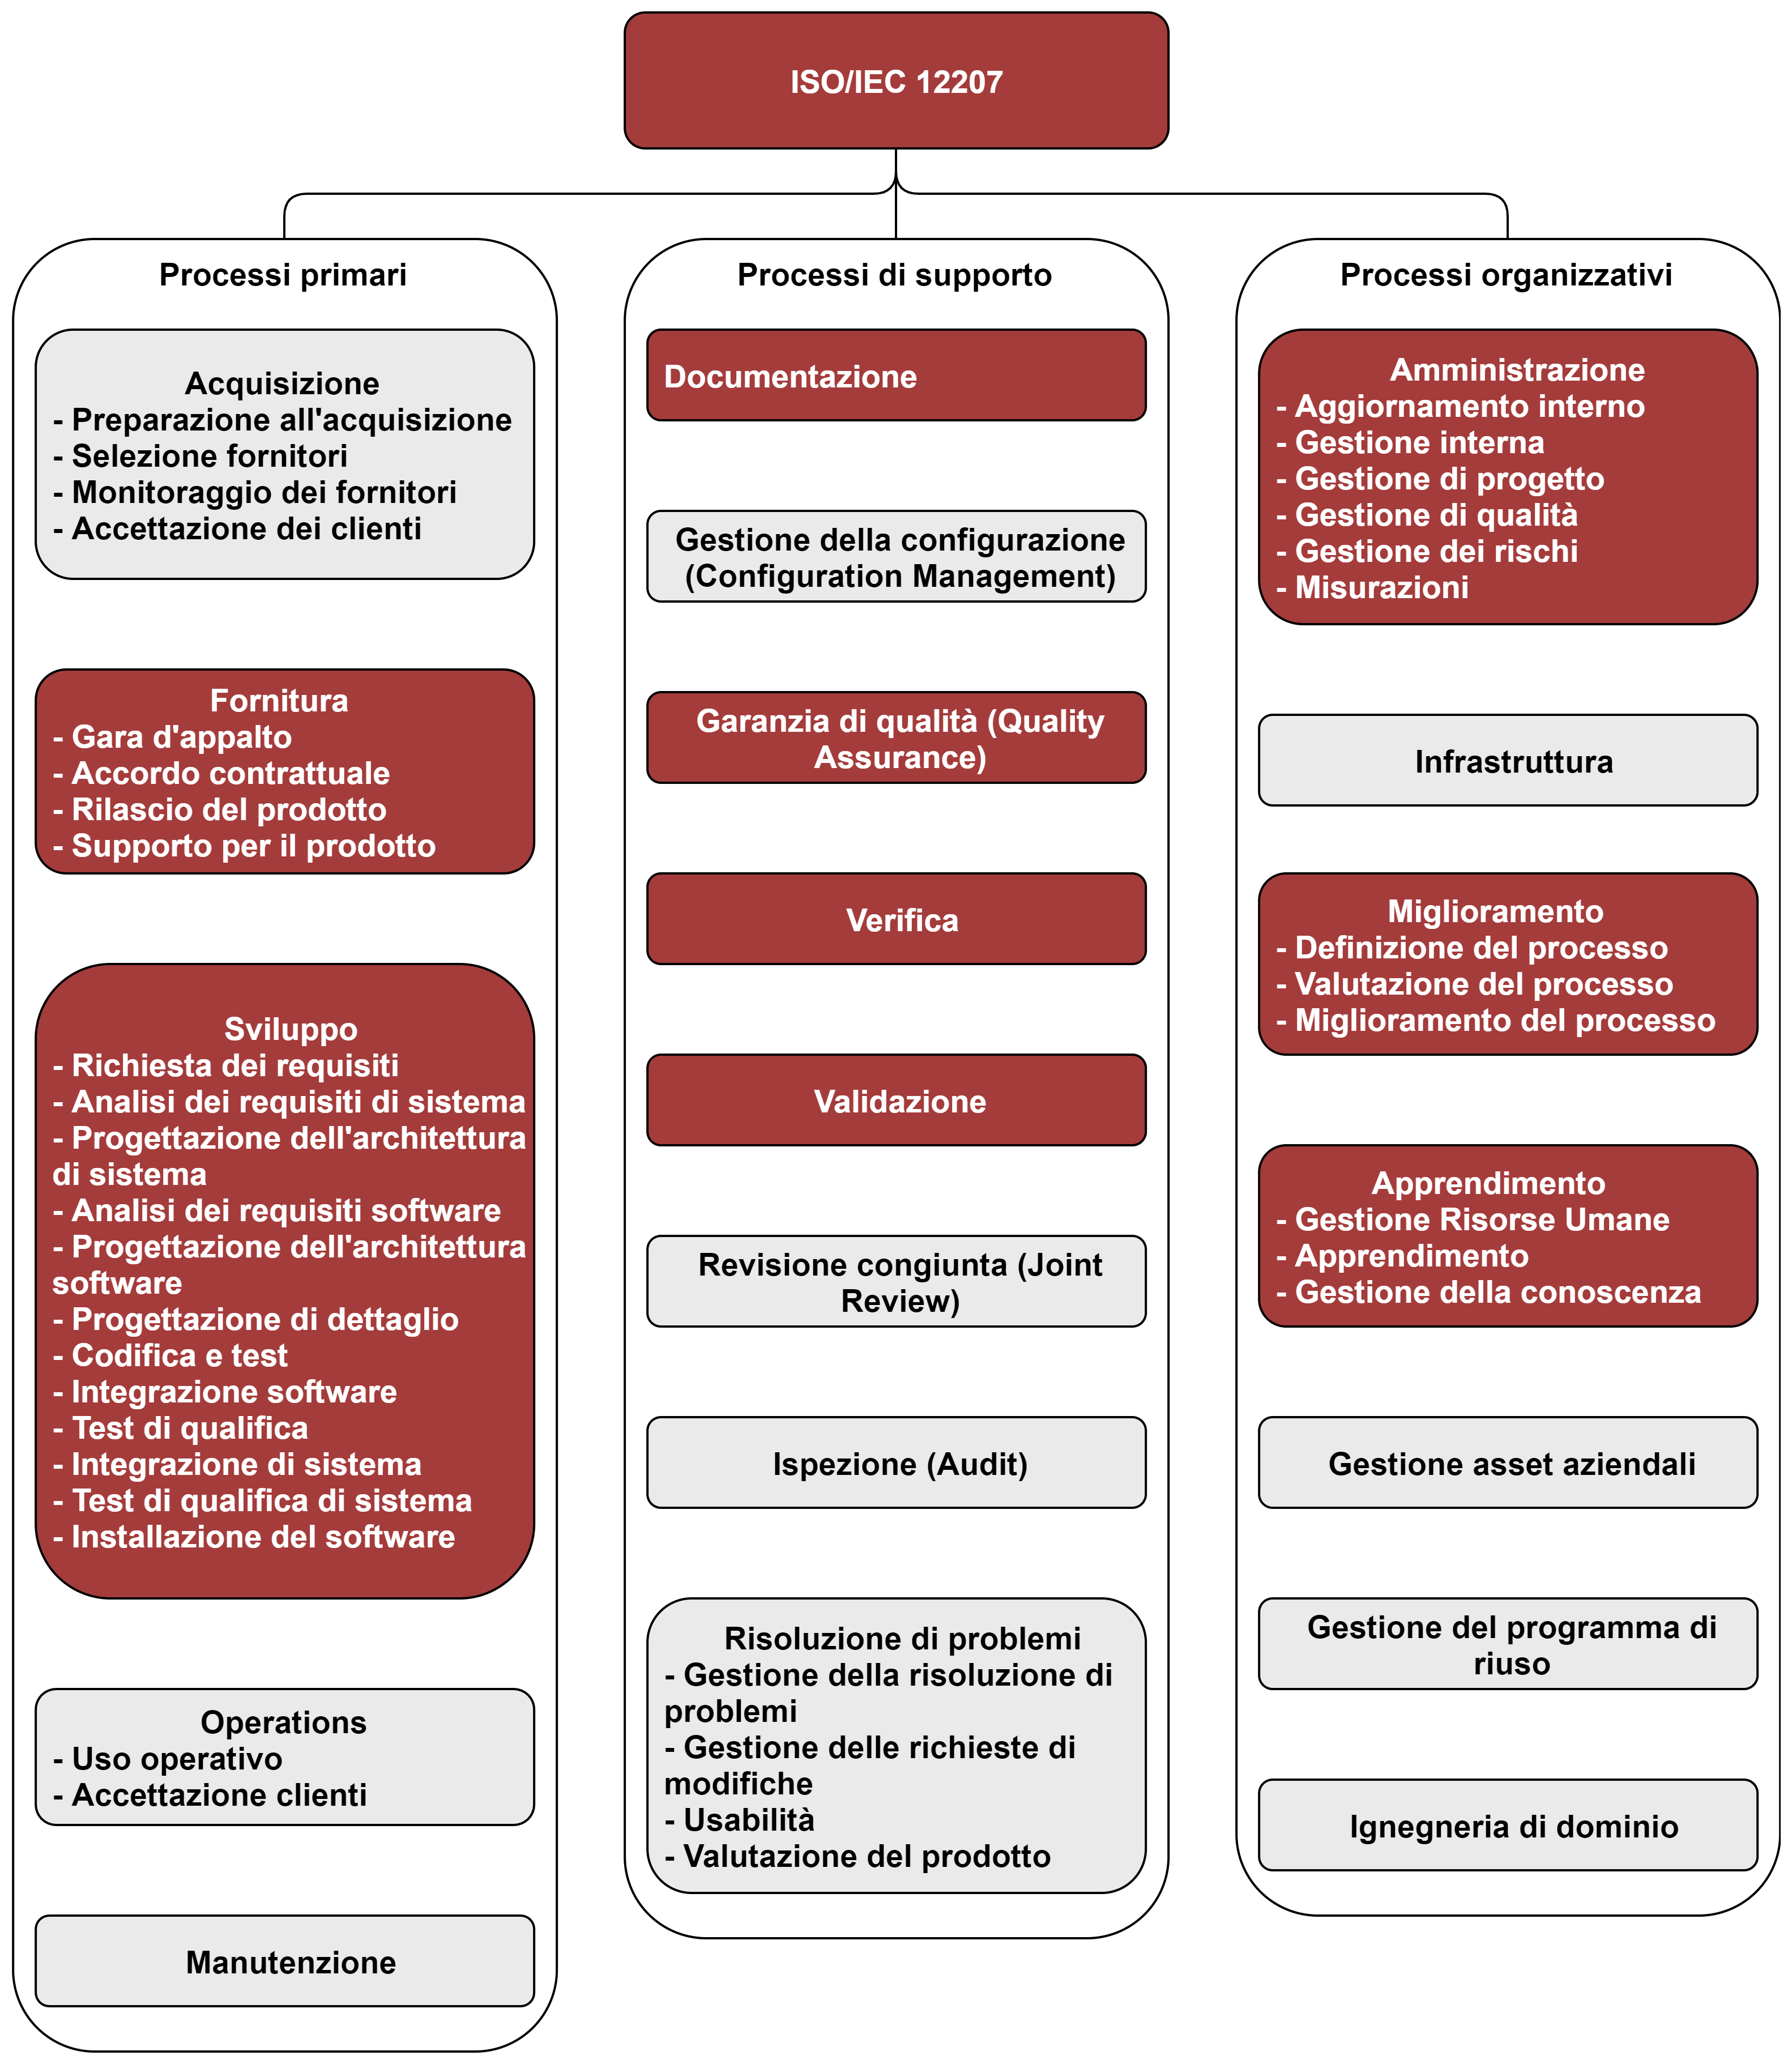
\includegraphics[scale=0.53]{Sezioni/Immagini/IsoIec12207.png}
    \caption{Schema dello standard ISO/IEC 12207. In rosso sono indicati i processi e le relative attività di interesse per il progetto.}
\end{figure}

\subsubsection{Processi primari}
Sono i \glo{processi} e le attività che fanno parte dello sviluppo del software e hanno lo scopo di soddisfare tutti i requisiti concordati con il cliente.

\paragraph{Sviluppo}\mbox{}\\ \\
Il \glo{processo} ha lo scopo di sviluppare un prodotto software, o un sistema basato sul software, che indirizzi le esigenze del cliente. \\
I risultati delle valutazioni dei \glo{processi} devono essere documentati.
\begin{itemize}
    \item \textbf{Analisi dei requisiti:} \\
    Lo sviluppatore deve valutare i requisiti software in base ai criteri elencati di seguito:
        \begin{itemize}
            \item Tracciabilità dei requisiti di sistema e progettazione del sistema;
            \item Coerenza esterna con i requisiti di sistema;
            \item Coerenza interna;
            \item \glo{Testabilità};
            \item Fattibilità della progettazione del software;
            \item Fattibilità di funzionamento e manutenzione.
        \end{itemize}
    \item \textbf{Pianificazione di dettaglio:} \\
    Lo sviluppatore deve sviluppare un progetto dettagliato per ciascun componente software. I componenti del software 
    devono essere perfezionati in livelli inferiori contenenti unità software che possono essere codificati, compilati 
    e testati. È necessario garantire che tutti i requisiti software siano assegnati dai componenti software 
    alle unità software.
    
    \item \textbf{Codifica:} \\
    Lo sviluppatore deve valutare il codice del software e i risultati dei test considerando i criteri elencati sotto:
    \begin{itemize}
        \item Tracciabilità ai requisiti e alla progettazione dell'articolo software;
        \item Coerenza esterna con i requisiti e il design dell'articolo software;
        \item Coerenza interna tra i requisiti dell'unità;
        \item Testare la copertura delle unità;
        \item Adeguatezza dei metodi e delle norme di codifica utilizzati;
        \item Fattibilità dell'integrazione e dei test del software;
        \item Fattibilità di funzionamento e manutenzione.   
    \end{itemize}
\end{itemize}

\subsubsection{Processi di supporto}
Sono i \glo{processi} e le attività che aiutano gli altri \glo{processi} nel raggiungimento del successo e nella qualità del progetto.

\paragraph{Documentazione}\mbox{}\\ \\
Il \glo{processo} di "Gestione della documentazione" garantisce lo sviluppo e la manutenzione delle informazioni prodotte e registrate relativamente al prodotto software. \\ \\
\textbf{Implementazione:} \\ 
Identifica i documenti da produrre durante il ciclo di vita del prodotto software;
deve essere sviluppato, documentato e implementato. La documentazione dovrà prevedere i seguenti punti: 
\begin{itemize}
    \item Titolo o nome;
    \item Scopo;
    \item Pubblico previsto;
    \item Procedure e responsabilità per input, sviluppo, revisione, modifica, approvazione, produzione, stoccaggio, distribuzione, manutenzione e gestione della configurazione;
    \item Programma per le versioni intermedie e finali.
\end{itemize}

\paragraph{Garanzia di qualità}\mbox{}\\ \\
Il \glo{processo} di "Assicurazione qualità" ha lo scopo di assicurare che tutti i prodotti di fase (work product) siano conformi con i piani e gli standard definiti.
\paragraph{Verifica}\mbox{}\\ \\
Il \glo{processo} di verifica ha lo scopo di confermare che ciascun work product o servizio realizzato da un \glo{processo} soddisfi i requisiti specificati. 
Il \glo{processo} di verifica deve essere integrato nei \glo{processi} di Sviluppo, Fornitura e Manutenzione. Se la verifica viene eseguita da terzi, questa viene definita come "\glo{Processo} di verifica indipendente".
\\
Il \glo{processo} deve essere verificato considerando i criteri elencati di seguito:
\begin{itemize}
    \item I requisiti di pianificazione del progetto sono adeguati e tempestivi;
    \item I \glo{processi} selezionati per il progetto sono adeguati, implementati, eseguiti come previsto, e conformi al contratto;
    \item Gli standard, le procedure e gli ambienti per i \glo{processi} del progetto sono adeguati;
    \item Il progetto è composto da personale qualificato capace di soddisfare le richieste del contratto.
\end{itemize}

\subsubsection{Processi organizzativi}
Sono i \glo{processi} e le attività che coprono gli aspetti organizzativi e di gestione delle risorse.

\paragraph{Gestione}\mbox{}\\ \\
Il \glo{processo} di gestione garantisce lo sviluppo e la manutenzione delle informazioni prodotte e registrate relativamente 
al prodotto software. L'amministratore prepara i piani per l'esecuzione del \glo{processo}.
I piani associati all'esecuzione del \glo{processo} devono contenere descrizioni: delle attività, dei compiti associati e
identificazioni dei prodotti software che verranno forniti. Questi piani devono rispettare i seguenti punti:
\begin{itemize}
    \item Programmi per il completamento tempestivo dei compiti;
    \item Risorse adeguate necessarie per eseguire i compiti;
    \item Assegnazione di compiti;
    \item Assegnazione di responsabilità;
    \item Quantificazione dei rischi associati ai compiti o al \glo{processo} stesso;
    \item Misure di controllo della qualità da applicare durante l'intero \glo{processo};
    \item Costi associati all'esecuzione del \glo{processo};
    \item Fornitura di ambiente e infrastruttura.
\end{itemize}

\subsection{ISO/IEC 9126}
Lo standard ISO/IEC 9126 si occupa di presentare le caratteristiche di qualità di un prodotto software e gli attributi che le compongono.

\begin{figure}[h]
    \centering
    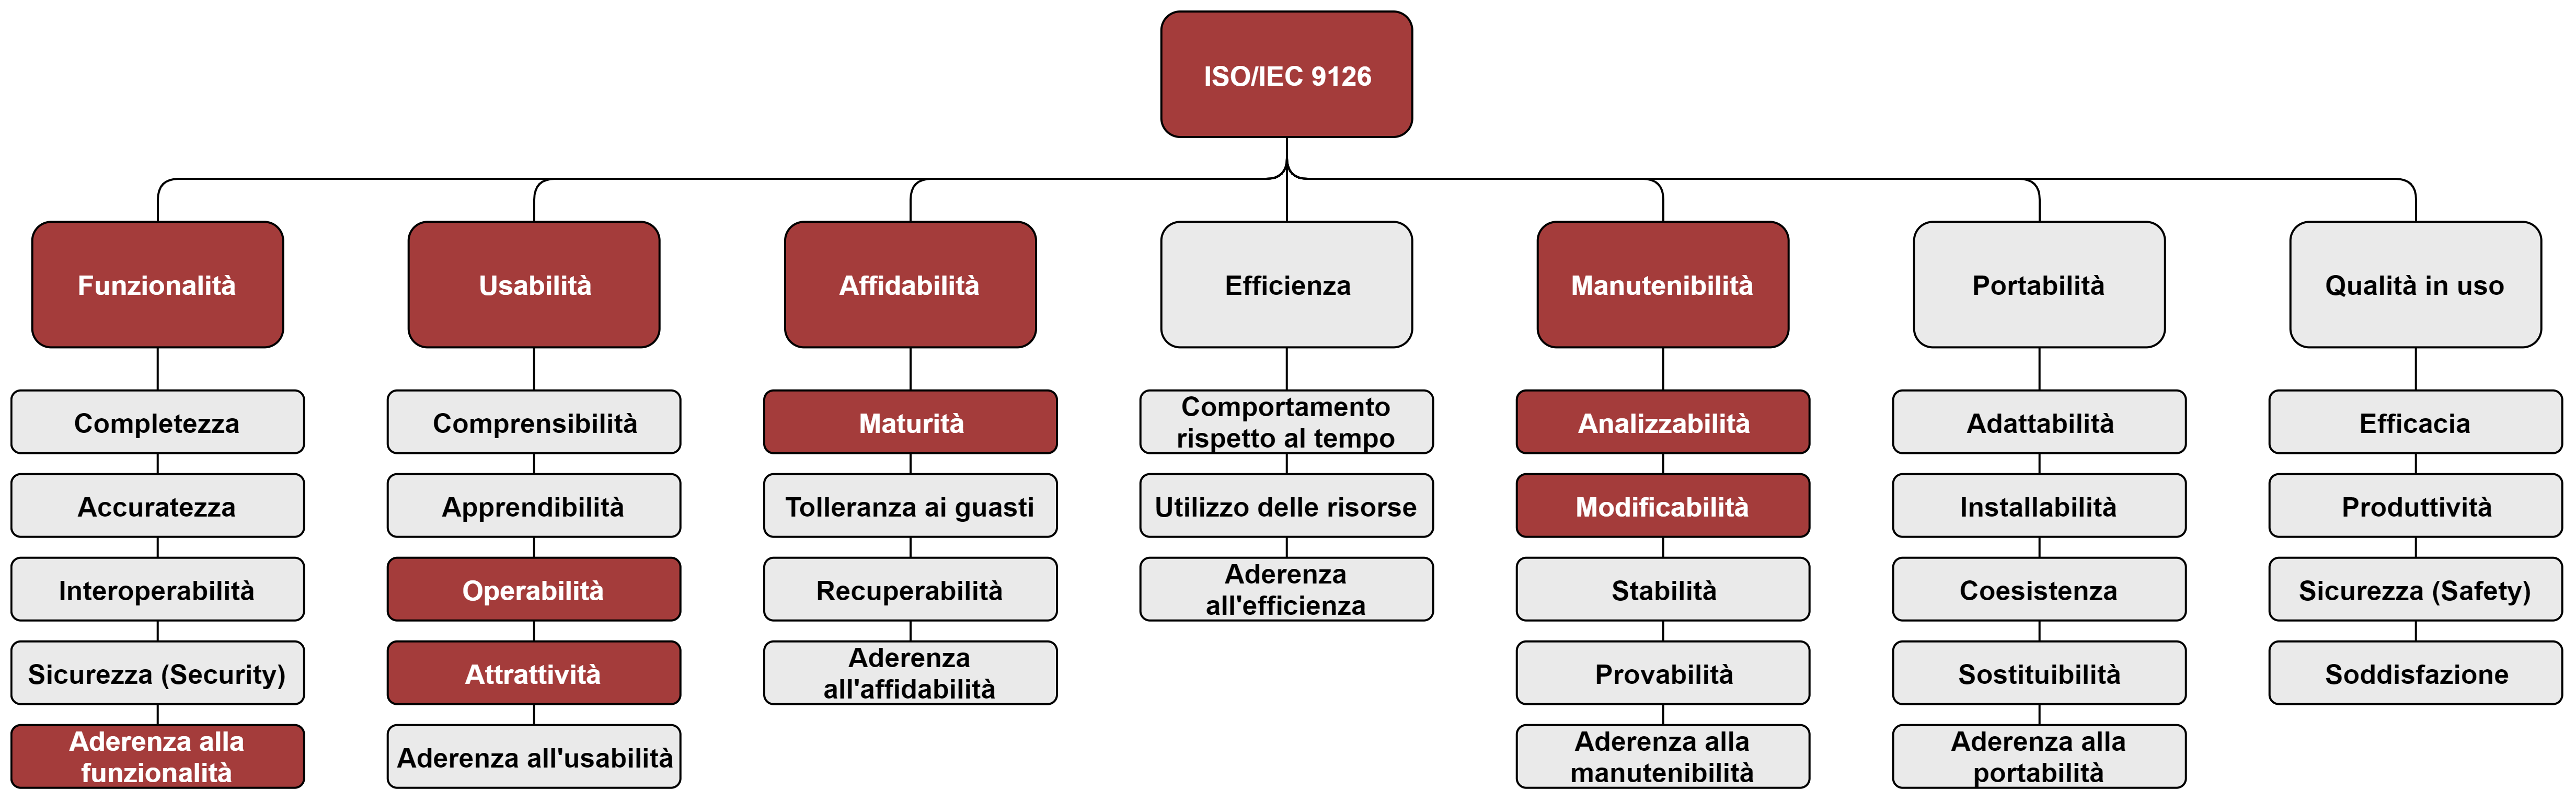
\includegraphics[scale=0.53]{Immagini/IsoIec9126.png}
    \caption{Schema dello standard ISO/IEC 9126. In rosso sono indicate le caratteristiche e attributi di interesse per il progetto.}
\end{figure}

\subsubsection{Metriche esterne}
Le metriche relative alla qualità "esterna" indirizzano le caratteristiche esteriori del software, cioè quelle rilevabili direttamente dagli utenti e dagli operatori.

\subsubsection{Metriche interne}
 Le metriche della qualità "interne" del software sono utilizzate durante la fase di sviluppo e permettono di valutare il comportamento del software dal punto di vista degli sviluppatori e di predire quello che sarà il punto di vista esterno degli utenti.

\subsubsection{Funzionalità}
Capacità del prodotto software di fornire funzioni adeguate al contesto di applicazione.
\begin{itemize}
\item \textbf{Adeguatezza}: Capacità di fornire un insieme di funzioni che permettano agli utenti del software di poter svolgere i loro compiti.
\item \textbf{Accuratezza}: Capacità di fornire i risultati attesi dall’utente con la precisione richiesta.
\item \textbf{Interoperabilità}: Capacità di interagire con uno o più sistemi specificati.
\item \textbf{Sicurezza (Security)}: Capacità di proteggere le informazioni e i dati dell’utente da persone non autorizzate ad accedervi.
\item \textbf{Aderenza alla funzionalità}: Capacità di aderire a standard, norme, convenzioni e regolamenti sulle funzionalità.
\end{itemize}

\subsubsection{Affidabilità}
Capacità del prodotto software di mantenere il livello di prestazione quando usato in condizioni specificate.
E’ limitata da errori nei requisiti, nella progettazione e nel codice del software.
\begin{itemize}
\item \textbf{Maturità}: Capacità di evitare che si verifichino errori.
\item \textbf{Tolleranza a guasti}: Capacità di mantenere il livello di prestazioni in caso di errori o violazione delle interfacce. Assieme alla \glo{Maturità}, descrivono l’attributo \glo{Disponibilità}, non specificato in quanto formato da questi due.
\item \textbf{Recuperabilità}: Capacità di ripristinare il livello di prestazioni e i dati in caso di errori e malfunzionamenti.
\item \textbf{Aderenza all’affidabilità}: Capacità di aderire a standard, norme, convenzioni e regolamenti sull’affidabilità.
\end{itemize}

\subsubsection{Usabilità}
Capacità del prodotto software di essere comprensibile, di poter essere studiato.
\begin{itemize}
\item \textbf{Comprensibilità}: Capacità di permettere all’utente di capire le funzionalità e come usarle con successo;
\item \textbf{Apprendibilità}: Capacità di permettere all’utente di imparare l’applicazione;
\item \textbf{Operabilità}: Capacità di permettere all’utente di usare il software e controllarlo;
\item \textbf{Attrattività}: Capacità di risultare attraente (ossia possedere una interfaccia utente accattivante);
\item \textbf{Aderenza all’usabilità}: Capacità di aderire a standard, norme, convenzioni e regolamenti sull’usabilità.
\end{itemize}

\subsubsection{Efficienza}
Capacità del prodotto software di realizzare le funzioni richieste nel minor tempo possibile.
\begin{itemize}
\item \textbf{Comportamento rispetto al tempo}: Capacità di fornire in tempi adeguati risposte per l’utente;
\item \textbf{Utilizzo risorse}: Capacità di utilizzare un appropriato numero e tipo di risorse, eseguendo le funzionalità previste;
\item \textbf{Aderenza all’efficienza}: Capacità di aderire a standard, norme, convenzioni e regolamenti sull’efficienza.
\end{itemize}

\subsubsection{Manutenibilità}
Capacità del prodotto software di essere modificato.
\begin{itemize}
\item \textbf{Analizzabilità}: Capacità di poter diagnosticare errori e individuare malfunzionamenti;
\item \textbf{Modificabilità}: Capacità di consentire lo sviluppo di modifiche al software originale;
\item \textbf{Stabilità}: Capacità di evitare effetti non desiderati;
\item \textbf{Provabilità}: Capacità di consentire la verifica delle funzionalità del prodotto software;
\item \textbf{Aderenza alla manutenibilità}: Vpacità di aderire a standard, norme, convenzioni e regolamenti sulla manutenibilità.
\end{itemize}

\subsubsection{Portabilità}
Capacità di essere trasportato da un ambiente ad un altro.
\begin{itemize}
\item \textbf{Adattabilità}: Verrà descritta se ce ne sarà il bisogno;
\item \textbf{Installabilità}: Verrà descritta se ce ne sarà il bisogno;
\item \textbf{Coesistenza}: Verrà descritta se ce ne sarà il bisogno;
\item \textbf{Aderenza alla portabilità}: Verrà descritta se ce ne sarà il bisogno.
\end{itemize}

\subsubsection{Qualità in uso}
\begin{itemize}
\item \textbf{Efficacia}: Capacità per l’utente del prodotto software di raggiungere obiettivi specifici con \glo{accuratezza} e \glo{completezza};
\item \textbf{Produttività}: Capacità di permettere all’utente di impegnare un numero definito di risorse, in relazione all’efficienza raggiunta. Queste risorse possono essere tempo, materiali e costi;
\item \textbf{Sicurezza fisica (Safety)}: Capacità di raggiungere un livello accettabile di rischio per dati, business e persone. I rischi sono tipicamente correlati a difetti in progettazione o analisi o codifica;
\item \textbf{Soddisfazione}: Capacità di soddisfare gli utenti in uno specifico contesto.
\end{itemize}
\newpage
\section{Resoconto delle attività di verifica}
In questa sezione vengono descritti ed analizzati gli esiti delle attività di verifica su tutti i documenti destinati alla consegna.

\subsection{Revisione dei requisiti}

\subsubsection{Analisi statica dei documenti}
I membri del gruppo \Gruppo{} hanno analizzato i documenti mediante la tecnica di walkthrough che ha portato all'individuazione di 
alcuni errori ortografici e grammaticali, grazie anche agli strumenti di controllo ortografico integrati negli editor per la produzione
della documentazione che il gruppo ha deciso di utilizzare.

\subsubsection{Esiti verifiche automatizzate}
Attualmente, l'unico valore che può essere calcolato per \glo{verificare} se la garanzia di qualità che il gruppo ritiene fornire è
soddisfatta, è data dall'Indice di Gulpease (MPC6).
%Per poter calcolare questo indice, viene utilizzato come strumento il "Calcolatore dell'Indice Gulpease" ospitato a \href{https://farfalla-project.org/readability_static/}{questo indirizzo}.
%Non vengono contati per l'indice di Gulpease il testo presente nelle seguenti parti o sezioni del documento:
%\begin{itemize}
  %  \item Indice;
  %  \item Registro delle modifiche;
  %  \item Riferimenti.
%\end{itemize}
Nella seguente tabella sono riportati i risultati degli indici di Gulpease ottenuti dai documenti per ogni periodo, successivamente ci sarà un grafico che riporterà l'andamento degli indici di Gulpease per ogni documento a seconda del periodo.

\paragraph{Legenda}
\begin{itemize}
	\item \textbf{Documento}: Nome del documento;
	\item \textbf{RR}: Periodo di revisione dei requisiti;
	\item \textbf{RP}: Periodo di revisione di progettazione;
	\item \textbf{RQ}: Periodo di revisione di qualifica;
	\item \textbf{RA}: Periodo di revisione di accettazione;
	\item \textbf{-}: Valore inesistente;
	\item  \textbf{Colore giallo}: Indica che il valore ottenuto è accettabile;
	\item  \textbf{Colore verde}: Indica che il valore ottenuto è ottimo. 
\end{itemize}
\newpage
{
\rowcolors{2}{grigetto}{white}
\renewcommand{\arraystretch}{1.5}
\centering
\begin{longtable}{C{4cm} C{1cm} C{1cm} C{1cm} C{1cm}}
\caption{Elenco dei indici di Gulpease }\\
\rowcolor{darkblue}
\textcolor{white}{\textbf{Documento}} & \textcolor{white}{\textbf{RR}} &
\textcolor{white}{\textbf{RP}} & \textcolor{white}{\textbf{RQ}} & 
\textcolor{white}{\textbf{RA}} \\
\hline
\endhead
\AdRv{1.0.0} & \textcolor{verde}{\textbf{95}} & - & - & -\\
\PdPv{1.0.0} & \textcolor{verde}{\textbf{100}} & - & - & -\\
\PdQv{1.0.0} & \textcolor{verde}{\textbf{100}} & - & - & - \\

\NdPv{1.0.0} & \textcolor{giallo}{\textbf{75}} & - & - & -\\
\SdFv{1.0.0} & \textcolor{verde}{\textbf{94}} & - & - & -\\

\Glossariov{1.0.0} & \textcolor{giallo}{\textbf{67}} & - & - & -\\

Media verbali interni & \textcolor{verde}{\textbf{92}} & - & - & -\\
Media verbali esterni & \textcolor{giallo}{\textbf{65}} & - & - & -\\

\end{longtable}

%\begin{figure}[h]
%	\centering
%	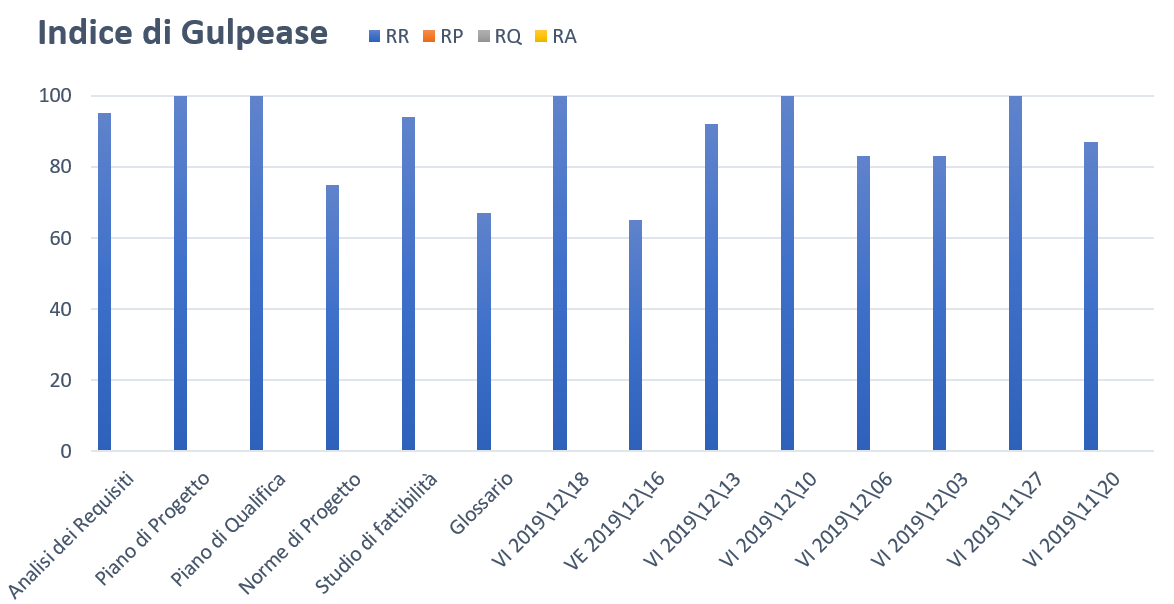
\includegraphics[scale=0.50]{Sezioni/Immagini/IG-Grafico.png}
%	\caption{Grafico andamento dell'Indice di Gulpease per ogni periodo e documento}
%\end{figure}
%}

\pgfplotsset{width=17cm, height=10cm}
\begin{tikzpicture}

\begin{axis}[
title=Grafico andamento dell'Indice di Gulpease per ogni periodo e documento,
x tick label style={
/pgf/number format/1000 sep=},
ylabel=Indice di Gulpease,
enlargelimits=0.05,
legend style={at={(0.5,-0.4)},
anchor=north,legend columns=-1},
ybar interval=0.5,
symbolic x coords={Analisi dei Requisiti, Piano di Progetto, Piano di Qualifica, Norme di Progetto, Studio di fattibilita, Glossario,
Media verbali interni, Media verbali esterni, tmp},%lasciare tmp come ultima colonna per poter visualizzare tutte le colonne tranne tmp
x tick label style={rotate=45,anchor=east},
xtick=data
]
\addplot[fill=blue] coordinates
{(Analisi dei Requisiti, 95) (Piano di Progetto, 100) (Piano di Qualifica, 100) 
(Norme di Progetto, 75) (Studio di fattibilita, 94) (Glossario, 67)
(Media verbali interni, 92) (Media verbali esterni, 65) (tmp, 0)};

\addplot [fill=orange] coordinates
{(Analisi dei Requisiti, 0) (Piano di Progetto, 0) (Piano di Qualifica, 0) 
(Norme di Progetto, 0) (Studio di fattibilita, 0) (Glossario, 0)
(Media verbali interni, 0) (Media verbali esterni, 0) (tmp, 0)};

\addplot [fill=gray] coordinates
{(Analisi dei Requisiti, 0) (Piano di Progetto, 0) (Piano di Qualifica, 0) 
(Norme di Progetto, 0) (Studio di fattibilita, 0) (Glossario, 0) 
(Media verbali interni, 0) (Media verbali esterni, 0) (tmp, 0)};
\addplot [fill=yellow] coordinates
{(Analisi dei Requisiti, 0) (Piano di Progetto, 0) (Piano di Qualifica, 0) 
(Norme di Progetto, 0) (Studio di fattibilita, 0) (Glossario, 0)
(Media verbali interni, 0) (Media verbali esterni, 0) (tmp, 0)};

\legend{
RR,
RP,
RQ,
RA
}
\end{axis}
\end{tikzpicture}
% \newpage
% \section{Riferimenti}

\subsection{Riferimenti normativi}
\begin{itemize}
\item \NdPv{1.0.0};
\item \textit{VE\_2019\_12\_13}.
\end{itemize}

\subsection{Riferimenti informativi}
\begin{itemize}
\item \SdFv{1.0.0};
\item \textbf{Slide del capitolato C5 - Stalker}: \\ \url{https://www.math.unipd.it/~tullio/IS-1/2019/Progetto/C5.pdf}
\item \textbf{Guide to the Software Engineering Body of Knowledge};
\item \textbf{Software Engineering (10th edition) - Ian Sommerville}.
\end{itemize}


\end{document}